%%%%%%%%%%%%%%%%%%%%%%%%%%%%%%%%%%%%%%%%%%%%%%%
%
% Template for Master degrees
% DISI - Department of Information Engineering and Computer Science
%
% update 2020-08-30
%
% To generate pdf 
% pdflatex __filename__.tex
% bibtex __file_name__.aux
% pdflatex __file_name__.tex
% pdflatex __file_name__.tex
%
%%%%%%%%%%%%%%%%%%%%%%%%%%%%%%%%%%%%%%%%%%%%%%%

% 2 side format
\documentclass[epsfig, a4paper, 11pt, titlepage, twoside, openany]{book}
\usepackage{epsfig}
\usepackage{plain}
\usepackage{setspace}
\usepackage{array}
\usepackage{afterpage}
\usepackage[paperheight=29.7cm, paperwidth=21cm, outer=1.5cm, inner=2.5cm, top=2cm, bottom=2cm]{geometry} % layout setting
\usepackage{titlesec} % custom setup title of chapter
% \usepackage{newtxtext,newtxmath} % times new roman
\usepackage{wrapfig}
\usepackage{float}
\usepackage{amstext}
\usepackage{amsmath}
\usepackage{enumitem}
\usepackage{multirow}
\usepackage{url}
%%%%%%%%%%%%%%
% support for accented letters
\usepackage[utf8]{inputenc}

\singlespacing

\usepackage[english]{babel}
\usepackage{chngcntr}
\counterwithout{footnote}{chapter}
\interfootnotelinepenalty=10000
\usepackage{subcaption}
\captionsetup{subrefformat=parens}

\usepackage[autostyle,italian=guillemets]{csquotes}
\usepackage[backend=bibtex, maxbibnames=10, style=numeric]{biblatex}
\addbibresource{bibliography.bib}

\begin{document}

  % no page number
  \pagenumbering{gobble} 
  \pagestyle{plain}

\thispagestyle{empty}

\vspace{1.2 cm}

\begin{center}
  \begin{figure}[h!]
    \centerline{
\psfig{file=images/misc/marchio_unitrento_colore_it_v2.eps,width=0.66\textwidth}}
  \end{figure}

  \vspace{0.5 cm}

  \LARGE{Department of Sociology and Social Research\\}

  \vspace{0.5 cm}
  \Large{Master's Degree in\\
    Data Science
  }

  \vspace{2.2 cm}
  \Large\textsc{Final Dissertation\\} 
  \vspace{1.2 cm}
  \Huge\textsc{Exploring the Feasibility and\\Effectiveness of Large Language\\Models for Automated Test Oracle\\Generation in Software Testing\\}
  % \Large{\it{Sub-title (optional)}}


  \vspace{2.2 cm}
  \begin{tabular*}{\textwidth}{ c @{\extracolsep{\fill}} c }
  \Large{\textbf{Supervisors}} & \Large{\textbf{Student}}\\
  \Large{Fitsum Meshesha Kifetew} & \Large{Shaker Mahmud Khandaker}\\
  \Large{Paolo Rota} & \\
  \end{tabular*}

  \vspace{2.2 cm}

  \Large{Academic year 2022/2023}
  
\end{center}

  \cleardoublepage
 
%%%%%%%%%%%%%%%%%%%%%%%%%%%%%%%%%%%%%%%%%%%%%%%%%%%%%%%%%%%%%%%%%%%%%%%%%%
%%%%%%%%%%%%%%%%%%%%%%%%%%%%%%%%%%%%%%%%%%%%%%%%%%%%%%%%%%%%%%%%%%%%%%%%%%
%% Note
%%%%%%%%%%%%%%%%%%%%%%%%%%%%%%%%%%%%%%%%%%%%%%%%%%%%%%%%%%%%%%%%%%%%%%%%%%
%% Thanks/ Acknowledgements section is optional
%%%%%%%%%%%%%%%%%%%%%%%%%%%%%%%%%%%%%%%%%%%%%%%%%%%%%%%%%%%%%%%%%%%%%%%%%%
%%%%%%%%%%%%%%%%%%%%%%%%%%%%%%%%%%%%%%%%%%%%%%%%%%%%%%%%%%%%%%%%%%%%%%%%%%
  \thispagestyle{empty}

\begin{center}
  {\bf \Huge Acknowledgments}
\end{center}

\vspace{4cm}

\noindent
\emph{Thanks to my parents and my family, who supported and facilitated me in all my studies.}

\noindent
\emph{Special thanks to all my grandparents for all they have done for me throughout my life journey.}

\vspace{\baselineskip}

\noindent
\emph{Heartfelt thanks to my girlfriend, who has been by my side with her emotional support and love which have never been lacking during my university career and beyond.}

\vspace{\baselineskip}

\noindent
\emph{Thanks to all my friends, classmates, and colleagues who have supported and helped me over the past three years.}

\vspace{\baselineskip}

\noindent
\emph{Thanks to my supervisors who made possible the realization of this thesis.}

\vspace{\baselineskip}

\noindent
\emph{Finally, thanks to myself for having managed to complete this study path despite working.}

  \clearpage
  \pagestyle{plain} % no heading, footer with centered page number
  \afterpage{\null\thispagestyle{empty}\clearpage}

  % page number with Arabic format
  \mainmatter

%%%%%%%%%%%%%%%%%%%%%%%%%%%%%%%%%%%%%%%%%%%%%%%%%%%%%%%%%%%%%%%%%%%%%%%%%%
%%%%%%%%%%%%%%%%%%%%%%%%%%%%%%%%%%%%%%%%%%%%%%%%%%%%%%%%%%%%%%%%%%%%%%%%%%
%% Note
%%%%%%%%%%%%%%%%%%%%%%%%%%%%%%%%%%%%%%%%%%%%%%%%%%%%%%%%%%%%%%%%%%%%%%%%%%
%% Length: approximately 70 pages.
%% These 70 pages include:
%%   table of contents
%%   abstract
%%   chapters
%% Exclude:
%%   title page
%%   acknowledgments
%%   bibliography
%%   attachments
%%%%%%%%%%%%%%%%%%%%%%%%%%%%%%%%%%%%%%%%%%%%%%%%%%%%%%%%%%%%%%%%%%%%%%%%%%
%%%%%%%%%%%%%%%%%%%%%%%%%%%%%%%%%%%%%%%%%%%%%%%%%%%%%%%%%%%%%%%%%%%%%%%%%%

    % index
    \tableofcontents
    \newpage
    \afterpage{\null\thispagestyle{empty}\clearpage}

    % group to define space between chapters
    \begingroup
      % no page break between chapters
      % override clear page commands
      %\renewcommand{\cleardoublepage}{} 
      %\renewcommand{\clearpage}{} 
      % override format of title chapter
      % from
      %   Chapter X
      %   Title
      % to
      %   X   Title
      
      \titleformat{\chapter}
        {\normalfont\Huge\bfseries}{\thechapter}{1em}{}
        
      \titlespacing*{\chapter}{0pt}{0.59in}{0.02in}
      \titlespacing*{\section}{0pt}{0.20in}{0.02in}
      \titlespacing*{\subsection}{0pt}{0.10in}{0.02in}
      
      % summary / abstract
      \chapter*{Abstract} % no number
\label{abtract}

\addcontentsline{toc}{chapter}{Abstract} % add to index
\vspace{0.4 cm}

Here goes the abstract....
      \newpage
      % \afterpage{\null\thispagestyle{empty}\clearpage}

%%%%%%%%%%%%%%%%%%%%%%%%%%%%%%%%%%%%%%%%%%%%%%%%%%%%%%%%%%%%%%%%%%%%%%%%%%
%%%%%%%%%%%%%%%%%%%%%%%%%%%%%%%%%%%%%%%%%%%%%%%%%%%%%%%%%%%%%%%%%%%%%%%%%%
%% Note
%%%%%%%%%%%%%%%%%%%%%%%%%%%%%%%%%%%%%%%%%%%%%%%%%%%%%%%%%%%%%%%%%%%%%%%%%%
%% The first chapter (abstract) of the final thesis must contain a summary of a 
%% maximum length of 3 pages, introducing the context and motivations,
%% resuming the problem faced by the student, the techniques used for the
%% investigation and the reached outcomes.
%% If the final thesis is developed in collaboration with other students,
%% the personal contribution of the student has to be underlined.
%%%%%%%%%%%%%%%%%%%%%%%%%%%%%%%%%%%%%%%%%%%%%%%%%%%%%%%%%%%%%%%%%%%%%%%%%%
%%%%%%%%%%%%%%%%%%%%%%%%%%%%%%%%%%%%%%%%%%%%%%%%%%%%%%%%%%%%%%%%%%%%%%%%%%      
      
      %%%%%%%%%%%%%%%%%%%%%%%%%%%%%%%%
      % chapters
      %
      % \input or \include

      \chapter{Introduction}
\label{cha:introduction}
\vspace{0.4 cm}

In the ever-evolving landscape of software development, ensuring the reliability and robustness of applications is a continuous pursuit. Software testing stands as a cornerstone of quality assurance, a meticulous process where developers manually create tests—guiding benchmarks known as test oracles—to determine if software behaves as intended. However, manual test oracle generation poses challenges—it's resource-intensive, error-prone, and struggles to keep pace with the dynamic evolution of software systems. To address these challenges, various automated test generation techniques have emerged, yet they too face limitations. Tools like EvoSuite rely on code implementation, and when errors exist in the code, generated tests may misconstrue these errors as actual behavior, leading to the Oracle problem in software testing.

Enter Large Language Models (LLMs), an exciting frontier in artificial intelligence. Trained on extensive natural language data, LLMs exhibit a unique ability to comprehend instructions and understand code contexts. This raises a compelling question: Can LLMs leverage their linguistic and coding knowledge to enhance the oracles of automatically generated tests?

In response to this inquiry, our thesis introduces EvoOracle—a groundbreaking tool designed to explore the intersection of LLMs and software testing. EvoOracle takes Java projects, extracts critical information, replaces assertions in test cases with placeholders, and harnesses the power of LLMs to generate precise assertions. The key innovation lies in the potential of LLMs to understand the expected behavior of code, transcending the limitations of traditional automated test generation tools. We embark on a comprehensive comparison with the EvoSuite baseline, aiming to showcase the transformative capabilities of LLMs in automating test oracle creation.

This journey delves into the synergy between machine learning and software testing, pushing the boundaries of what's possible in enhancing software reliability. Through meticulous experimentation and evaluation, we seek to unravel the true potential of LLMs in redefining the future of software testing. Our work not only addresses the Oracle problem but also opens avenues for broader applications of LLMs in the realm of software engineering. In conclusion, this thesis embarks on a journey into the future of software testing, where Large Language Models emerge as intelligent allies in the pursuit of software reliability and innovation. Our work holds the potential to redefine software quality assurance, offering a glimpse into a world where artificial intelligence meets code-centric domains, promising a future where software correctness is achieved with unprecedented ease and precision. 

The thesis unfolds in a structured manner, offering an insightful journey into the realms of Large Language Models (LLMs) and their application in automated test oracle generation. In Chapter~\ref{cha:background}, we lay the foundation with a detailed exploration of LLMs, delving into their underlying concepts and significance. Simultaneously, we scrutinize the landscape of software testing and the crucial role of test oracles, setting the stage for the challenges addressed in this research. Additionally, we navigate through the landscape of automated test generation, identifying existing methodologies and their limitations. For readers already acquainted with these concepts, a smooth transition to Chapter~\ref{cha:state_of_the_art} is encouraged, as it builds upon this foundational knowledge.

Chapter~\ref{cha:state_of_the_art} unfurls as a comprehensive canvas with a methodology for identifying relevant papers, ensuring a robust literature review. This chapter meticulously examines the state of the art in oracle generation and unit test generation, providing a backdrop for the innovative approaches proposed in this thesis.

The core of our exploration unfolds in Chapter~\ref{cha:evoOracles}, where we delve into the practical implementation of LLMs for oracle generation. The journey begins with a detailed account of data collection from Java projects, incorporating the intricate process of test case generation using EvoSuite. Subsequently, we navigate through preprocessing steps, including the removal of assertions, placeholder insertion, and the intricate integration of LLMs into the testing workflow. Each step is methodically detailed, offering transparency into our experimental design.

Chapter~\ref{cha:experiments} serves as the crucible of experimentation, outlining the experimental setup, research questions, and the meticulous evaluation of results. We embark on a rigorous analysis of the effectiveness and efficiency of LLMs, answering critical research questions and addressing potential threats to validity. This chapter forms the empirical backbone, substantiating the transformative potential of LLM-driven test oracle generation.

In the concluding chapter, Chapter~\ref{cha:conclusions}, we distill the essence of our findings, summarizing key insights and their implications. We outline avenues for future research, shedding light on the broader implications of our work in the domain of software testing and beyond.
      \newpage
      \afterpage{\null\thispagestyle{empty}\clearpage}

      \chapter{Background}
\label{cha:background}
\vspace{0.4 cm}

This chapter contains background information on the most relevant topics in this thesis: Large Language Models (LLMs), Software Testing and Test Oracle, Automated Test Generation.
Software development has evolved into a cornerstone of modern society, powering an array of applications from communication and commerce to healthcare and entertainment. This ubiquity underscores the critical importance of software quality and reliability. In the quest for robust software, software testing plays a pivotal role. The effectiveness of testing largely hinges on the concept of a "test oracle," which serves as a benchmark for assessing whether software behaves as expected.

\section{Large Language Models (LLMs)}
\label{sec:llms}
\vspace{0.2 cm}

Large language models (LLMs) represent a remarkable breakthrough in deep learning for natural language processing. They are capable of understanding and generating text in a manner that closely resembles human language comprehension. Behind the scenes, these LLMs are powered by extensive transformer models, which serve as the driving force behind their impressive capabilities.

While humans perceive text as collections of words, sentences, and documents, computers view text as mere sequences of characters. To bridge this gap, recurrent neural networks were initially employed to process text, operating one word or character at a time. However, they often struggled with retaining information from the beginning of a sequence when reaching the end.

In 2017, Vaswani et al. introduced the "Attention is All You Need"\cite{vaswani_attention_2017} paper, which laid the foundation for the transformer model. This revolutionary model leverages the attention mechanism, allowing it to process entire sentences or paragraphs at once, rather than one word at a time. This shift enables the transformer model to grasp the context of a word more effectively, leading to superior language understanding. Many cutting-edge language processing models are now based on transformers.

To utilize a transformer model for text processing, the first step involves tokenizing the text into a sequence of words. These tokens are then encoded as numerical values and transformed into embeddings, which are vector representations preserving the meaning of the tokens. Subsequently, the transformer's encoder transforms these token embeddings into a context vector, encapsulating the essence of the entire input. Using this vector, the transformer's decoder generates output based on contextual clues. For example, providing the original input as a clue allows the decoder to produce the next word in a sentence naturally. This process can be repeated to generate entire paragraphs, starting from an initial sentence—a method known as autoregressive generation. Large language models utilize transformer models capable of handling lengthy input texts, generating complex concepts with their extensive encoder and decoder layers.

Large language models, such as the GPT-3 model supporting ChatGPT, are built on an extensive scale. They are so massive that they cannot run on a single computer and are typically offered as services through APIs or web interfaces. These models are trained on vast amounts of text data from the internet, encompassing books, articles, websites, and diverse sources. During training, the model learns the statistical relationships between words, phrases, and sentences, enabling it to generate coherent and contextually relevant responses to prompts or queries.

Drawing from this wealth of text, GPT-3, for example, exhibits multilingual capabilities and possesses knowledge across various topics. This versatility allows it to produce text in various styles. Leveraging this, large language models can perform tasks like translation, text summarization, question answering and sentiment analysis. They have become valuable tools for automating language-related tasks, simplifying content generation, and enhancing human-computer interaction. Beyond their natural language capabilities, LLMs are increasingly being explored in the realm of software engineering. Their proficiency in understanding programming languages and code-related contexts has opened doors to innovative applications in software development, code generation, and, notably, software testing.

\textbf{TODO}\\
Write about key concepts of LLMs used in this thesis.

\section{Software Testing and Test Oracle}
\label{sec:software_testing_and_oracle}
\vspace{0.2 cm}

Software testing emerges as the sentinel, guarding against the unseen complexities that may lurk within code. It is the systematic process of evaluating software to ensure that it behaves as intended and meets the specified requirements. Let us go through some of the key components and concepts of software testing.

\begin{itemize}
  \item \textbf{Test Case:} Imagine a test case as a set of predefined actions and inputs meticulously crafted to assess a specific aspect of software functionality. Test cases serve as the evaluative criteria, scrutinizing the software under different scenarios. A JUnit test case typically follows a structure that includes the following components:

    \begin{enumerate}
        \item \textbf{Annotations:} \\
        - \textit{@Test}: Indicates that the method is a test method. \\
        - Other annotations like \textit{@Before, @After, @BeforeClass}, and \textit{@AfterClass} may also be used for setup and teardown operations.

        \item \textbf{Test Method:} \\
        - Contains the actual test logic that needs to be verified. \\
        - It is annotated with \textit{@Test}. \\
        - It often includes assertions to check whether the expected results match the actual results.

        \item \textbf{Setup and Teardown Methods (Optional):} \\
        - \textit{@Before}: Executed before each test method. It is used for setting up preconditions. \\
        - \textit{@After}: Executed after each test method. It is used for cleaning up resources. \\
        - \textit{@BeforeClass}: Executed once before any of the test methods in the class. It is used for expensive setup. \\
        - \textit{@AfterClass}: Executed once after all the test methods in the class have been run. It is used for cleanup after all tests.

        \item \textbf{Assertions:} \\
        - Used to verify whether the expected outcomes match the actual outcomes. \\
        - Commonly used methods\cite{noauthor_assert_nodate} include "assertEquals", "assertTrue", "assertFalse", "assertNotNull", "assertNull", etc.
    \end{enumerate}
  
  \item \textbf{Test Suite:} A collection of individual test cases forms a test suite. Test suites encompass diverse scenarios, covering a spectrum of functionalities to comprehensively evaluate the software.
  \item \textbf{Bug:} A bug, often referred to as a defect or issue, denotes an unintended and erroneous behavior within the software. The goal of testing is to unearth these bugs, enabling developers to rectify them before the software reaches end-users.
  \item \textbf{Test Oracle:} The Test Oracle is a critical entity that determines whether the software under examination 
  has exhibited the expected behavior. Think of it as the judge in a courtroom, rendering a verdict on whether the software stands acquitted or if discrepancies, i.e., bugs, have been found. It encapsulates the specifications, requirements, and expected results against which the software's performance is evaluated.
  \item \textbf{Unit testing:} Unit testing is the bedrock of software quality assurance, focusing on evaluating individual units or components of code in isolation. Each unit, typically a function or method, undergoes a battery of test cases designed to validate its correctness, functionality, and conformity to specifications. The goal is to ensure that these units operate as intended and integrate seamlessly within the broader software architecture. Unit testing facilitates early bug detection, fosters code maintainability, and forms an integral part of the test-driven development (TDD) methodology.
  \item \textbf{Line coverage:} Line coverage stands as a quantitative measure gauging the extent to which individual lines of code are exercised during testing. It represents the ratio of executed lines to the total lines in the codebase, providing insights into the effectiveness of test suites. While line coverage offers a valuable metric for assessing code exploration, it doesn't guarantee comprehensive testing, as it solely focuses on the presence or absence of executed lines, overlooking potential edge cases and conditional scenarios.
  \item \textbf{Mutation testing:} Mutation testing injects controlled defects, or mutations, into the codebase to evaluate the efficacy of test suites in detecting these alterations. Each mutation introduces a subtle change, simulating a potential bug. The ability of test suites to identify and flag these mutations reflects their robustness. This technique goes beyond traditional coverage metrics, assessing the quality of tests by evaluating their sensitivity to subtle code variations.
  \item \textbf{Mutation coverage:} Mutation coverage quantifies the proportion of mutations that test suites successfully detect. It serves as a qualitative measure, indicating the thoroughness of testing in identifying and isolating potential defects. A high mutation coverage suggests that the test suite is adept at pinpointing code alterations, enhancing confidence in the software's resilience against subtle bugs and ensuring comprehensive testing across diverse scenarios.
  \item \textbf{Test strength:} Test strength encapsulates the effectiveness of a test suite in uncovering defects and ensuring software reliability. It considers factors such as the diversity of test cases, their ability to explore different code paths, and their capacity to reveal potential vulnerabilities. A robust test suite exhibits high test strength, providing a solid defense against bugs and contributing to the overall quality assurance strategy.
  
\end{itemize}



\section{Automated Test Generation}
\label{sec:automated_test_generation}
\vspace{0.2 cm}

Historically, test oracles have been constructed manually by human testers, inspecting software outputs against expected results. While effective, this approach is labor-intensive and prone to human error. Automation techniques have been developed to alleviate this burden. Automation not only reduces the resources required for testing but also enhances test coverage by enabling the generation of a large number of test cases with minimal human intervention.

Automated test generation techniques leverage various algorithms and heuristics to generate test cases automatically. These techniques can be categorized into model-based, search-based, and \\
specification-based approaches. Model-based methods create models of the software's behavior, while search-based approaches explore the input space to find test cases that trigger specific conditions. Specification-based methods rely on formal specifications to guide test case generation.

\textbf{The Oracle Problem:}
In the context of automated testing, the Oracle Problem refers to the challenge of accurately determining expected outcomes. If the criteria for expected behavior are flawed, the automated testing tool may inadvertently accept erroneous behaviors as correct. 
Software systems are dynamic, subject to frequent updates, enhancements, and modifications. These changes ripple through the entire ecosystem, impacting functionalities and potentially altering expected outcomes. Maintaining a static set of expected outcomes becomes arduous. As the software evolves, the Oracle must dynamically adapt to these changes, requiring a level of agility that traditional testing approaches struggle to achieve. Defining precise criteria for expected behavior in complex software systems is inherently intricate. It involves considering a multitude of variables, interactions, and potential scenarios, often surpassing human capacity for manual formulation. Traditional automated testing tools often rely on predefined algorithms or criteria to determine expected outcomes. Crafting algorithms that encapsulate the nuanced behavior of diverse functionalities poses a considerable technical challenge, especially in scenarios where the desired outcome may not have a deterministic definition. The Oracle must possess adaptability and resilience to handle unforeseen circumstances. Traditional oracles, lacking the ability to dynamically adapt, may falter in scenarios where predefined criteria are insufficient to encompass the entire spectrum of possible outcomes.

Understanding the technical nuances of the Oracle Problem sets the stage for exploring innovative solutions, such as leveraging Large Language Models (LLMs), to navigate the intricacies of automated testing in contemporary software landscapes.
      \newpage
      % \afterpage{\null\thispagestyle{empty}\clearpage}
      
      \chapter{State of the Art}
\label{cha:state_of_the_art}
\vspace{0.4 cm}

In this chapter, we present a comprehensive exploration of the current state of the art within the domain of automated test oracle generation and the application of Large Language Models in software testing. We initiate our journey by introducing the foundational concepts and standards that underpin the representation of software testing data, with a specific focus on the intricacies of test oracles. Subsequently, we delve into an extensive survey of cutting-edge technologies and methodologies proposed in the literature for automated test oracle generation. This survey encompasses a wide spectrum of implementations and use cases, offering a panoramic view of the advancements in this field. As our journey unfolds, we shine a spotlight on two pivotal subjects that have garnered significant attention and innovation in the research community: Oracle generation and Unit Test Generation. These topics are not merely explored but dissected in dedicated subsections, elucidating their relevance and implications in the context of test oracle generation. Furthermore, we narrow our gaze to scrutinize the intricate nuances of three distinct yet interrelated use cases, each of paramount importance: automated test oracle generation for functional testing, regression testing, and security testing. These dedicated sections unravel the intricacies of generating test oracles that cater to the specific requirements and challenges posed by each testing domain. By the end of this chapter, a clear and comprehensive context will be established, providing the foundation upon which our proposed system for automated test oracle generation is developed. The synthesis of insights from literature, advancements in technology, and an understanding of the unique challenges in the realm of software testing will pave the way for a novel and effective approach that leverages Large Language Models to elevate the field of software quality assurance.


\section{Methodology for Identifying Relevant Papers}
\label{sec:papaer_survey_methodology}
\vspace{0.2 cm}

In this section, we describe the methodology that we followed to identify relevant papers for our study. We conducted this survey to collect scientific literature at the crossroads of software testing and large language models. Our search strategy aimed for a broad search string that encompasses various ways researchers might mention work related to oracle generation with large language models, as explained below:

\begin{enumerate}[label=\textbf{\arabic*.}]
  \item\textbf{Initial search and first-stage filtering.} We began our search in the SciVerse Scopus digital library\cite{Elsevier} by using the following search string. We chose all papers whose title, abstract, or keywords aligned with any of the keywords in the query:

  \textit{( TITLE-ABS-KEY( "software testing" OR "software verification" OR "software validation" OR "test case generation" OR "test suite generation" OR "test generation" OR "mutation testing" OR "fuzz testing" OR "property-based testing" OR "symbolic execution" OR "oracle" OR "assertion" ) AND TITLE-ABS-KEY ( "language model*" OR "transformer model*" ) )}

  We started our search with a broad query in the SciVerse Scopus digital library and got 191 studies initially. We performed this search on 18 May 2023, 16:51:58. Since the query was broad, the initial set had papers not related to Software Testing and Large Language Models. It included various types of artifacts like research articles, editorials, standards, and welcome messages. To refine our selection, we manually reviewed titles and abstracts, removing papers clearly unrelated to Software Testing and LLMs, as well as irrelevant artifacts. After this, we ended up with a final set of 37 studies.
  
  \item\textbf{Selection criteria.} We further filtered the collected papers based on certain rules to keep only the ones directly related to software testing with large language models. We excluded papers that didn't focus on either software testing or large language models. The papers we kept had to meet specific criteria:
      \begin{itemize}
            \item \textbf{Inclusion Criterion 1:} The study should involve defining, applying, or experimenting with software testing solutions using large language models.
            \item \textbf{Inclusion Criterion 2:} It presents an empirical or experimental study exploring the use of LLMs in software testing practices.
            \item \textbf{Inclusion Criterion 3:} The paper applies LLMs to various tasks within the software testing lifecycle.
            \item \textbf{Inclusion Criterion 4:} The study should have undergone peer review.
            \item \textbf{Inclusion Criterion 5:} The study should be written in English.
            
      \end{itemize}

  We excluded papers that meet at least one of the following exclusion criteria:
        \begin{itemize}
            \item \textbf{Exclusion Criterion 1:} Papers that don't involve software testing tasks, such as code comment generation.
            \item \textbf{Exclusion Criterion 2:} Papers that don't use Large Language Models (LLMs).
            \item \textbf{Exclusion Criterion 3:} Papers mentioning LLMs only in future work or discussions rather than actively using LLMs in their approach.
            \item \textbf{Exclusion Criterion 4:} Studies conducted before 2015.
            \item \textbf{Exclusion Criterion 5:} Secondary or tertiary studies, such as systematic literature reviews and surveys.
            \item \textbf{Exclusion Criterion 6:} Studies not available as full-text.
      \end{itemize}
At this stage, we ended up with a total of 8 papers related to our topic.

  \item\textbf{Snowballing.} We finalized our study selection using a snowballing approach. We conducted a thorough backward snowballing, examining references in the chosen studies and adding relevant papers from major databases such as SciVerse Scopus, IEEEXplore\cite{noauthor_ieee_nodate}, and ACM DL\cite{noauthor_acm_nodate}. After applying inclusion and exclusion criteria, we added three new papers, concluding with a set of 11 studies presented in Table \ref{tab:collected_papers} for our survey.
\end{enumerate}

\begin{table}[H]
\centering


    \begin{tabular}{c|c|c|c|c}
        \textbf{ID} & \textbf{Topic} & \textbf{Paper Title} & \textbf{Year} & \textbf{Reference}\\
        \hline 
        1 & \scriptsize\textsc{Oracle Generation} & \scriptsize\textsc{TOGA: A Neural Method for Test Oracle Generation} & 2022 & \cite{gabriel_ryan_toga_2022}\\
        
        2 & \scriptsize\textsc{Oracle Generation} & \scriptsize\textsc{Generating accurate assert statements for unit test} & 2022 & \cite{tufano_generating_2022}\\
        & & \scriptsize\textsc{cases using pretrained transformers} & & \\
        
        3 & \scriptsize\textsc{Oracle Generation} & \scriptsize\textsc{Automated assertion generation via information} & 2022 & \cite{yu_automated_2022}\\
        & & \scriptsize\textsc{retrieval and its integration with deep learning} & & \\
        
        4 & \scriptsize\textsc{Oracle Generation} & \scriptsize\textsc{Learning Deep Semantics for Test Completion} & 2023 & \cite{nie_learning_2023}\\

        5 & \scriptsize\textsc{Oracle Generation} & \scriptsize\textsc{Towards More Realistic Evaluation for} & 2023 & \cite{liu_towards_2023}\\
        & & \scriptsize\textsc{Neural Test Oracle Generation} & & \\
        
        6 & \scriptsize\textsc{Unit Test Generation} & \scriptsize\textsc{Unit Test Case Generation with Transformers} & 2021 & \cite{tufano_unit_2021}\\
        & & \scriptsize\textsc{and Focal Context} & & \\
        
        7 & \scriptsize\textsc{Unit Test Generation} & \scriptsize\textsc{Adaptive Test Generation Using a Large} & 2023 & \cite{schafer_adaptive_2023}\\
        & & \scriptsize\textsc{Language Model} & & \\
        
        8 & \scriptsize\textsc{Unit Test Generation} & \scriptsize\textsc{ChatUniTest: a ChatGPT-based automated unit} & 2023 & \cite{xie_chatunitest_2023}\\
        & & \scriptsize\textsc{test generation tool} & & \\
        
        9 & \scriptsize\textsc{Unit Test Generation} & \scriptsize\textsc{No More Manual Tests? Evaluating and Improving} & 2023 & \cite{yuan_no_2023}\\
        & & \scriptsize\textsc{ChatGPT for Unit Test Generation} & & \\
        
        10 & \scriptsize\textsc{Unit Test Generation} & \scriptsize\textsc{ChatGPT vs SBST: A Comparative Assessment of} & 2023 & \cite{tang_chatgpt_2023}\\
        & & \scriptsize\textsc{Unit Test Suite Generation} & & \\
        
        11 & \scriptsize\textsc{Unit Test Generation} & \scriptsize\textsc{CodaMosa: Escaping Coverage Plateaus in Test} & 2023 & \cite{lemieux_codamosa_2023}\\
        & & \scriptsize\textsc{Generation with Pre-trained Large Language Models} & & \\
        
    \end{tabular}

\caption{Details of the collected papers.}
\label{tab:collected_papers}
\end{table}

\section{Oracle Generation}
\label{sec:soa_oracle_generation}
\vspace{0.2 cm}

Gabriel Ryan et al. introduce TOGA\cite{gabriel_ryan_toga_2022}, an innovative contribution to the domain of Test Oracle Generation. This comprehensive framework comprises distinct components, including an Exceptional Oracle Classifier, trained on Methods2Test\cite{noauthor_unit_2023}, an Assertion Oracle Ranker trained on Atlas, and Candidate Assertion Set Generation, aided by both a Global Constant Dictionary and a Local Dictionary. TOGA's integration with EvoSuite enhances its versatility, providing a test prefix and unit context. The authors address pivotal research questions, demonstrating the effectiveness of TOGA in both grammar representation and the inference of assertions and exceptional behavior. Their results showcase TOGA's accuracy, surpassing existing methods in oracle inference and revealing its potential to uncover a substantial number of real-world bugs, including those missed by other approaches. The contributions encompass the introduction of a transformer-based approach, adapted datasets, and an end-to-end integration with EvoSuite, all of which significantly advance the field of test oracle generation. While the study acknowledges potential threats to validity, the TOGA framework's multifaceted capabilities demonstrate a promising direction for automated test oracle generation in software testing research.

Tufano et al. present an innovative contribution\cite{tufano_generating_2022} to Test Oracle Generation, focusing on the accurate generation of assert statements for unit test cases using pretrained transformers. Their framework, comprising the BART Transformer, English and Code Pretraining, and Asserts Finetuning, demonstrates significant advancements in this domain. Addressing key research questions, their approach excels when compared to ATLAS, achieving a remarkable 80\% relative improvement in top-1 accuracy. The study also explores the impact of pretraining on assert generation tasks, revealing substantial performance gains attributed to English and source code pretraining. The incorporation of the Focal Method contributes to a notable improvement in assert generation accuracy. Furthermore, the paper highlights the quality of the generated assert statements, demonstrating the model's ability to generate complex assertions akin to developer-authored ones. Notably, their approach can be employed to enhance automatically generated test cases, improving test coverage by augmenting existing cases. The dataset, drawn from a diverse range of sources including English text and GitHub, underscores the empirical rigor of their research. While addressing potential threats to validity, the paper underscores the potential of pretrained transformers in revolutionizing test oracle generation, promising substantial advancements in the generation of accurate assert statements and the augmentation of test cases.

Nie et al. introduce a novel approach TECO\cite{nie_learning_2023}, aimed at aiding developers in the efficient creation of test methods. Their groundbreaking approach, leverages code semantics and execution processes in machine learning models for code-related tasks. TECO, a transformer model trained on extensive code semantics data, demonstrates exceptional performance on the test completion task. It surpasses all baseline models by a significant margin, achieving an impressive exact-match accuracy of 17.61\%, a 29\% improvement over the best baseline. TECO not only generates compilable and runnable statements with high success rates but also excels in other metrics measuring lexical similarity. Moreover, the paper highlights TECO's impact on test oracle generation, showcasing an 82\% enhancement in exact-match accuracy over the prior state-of-the-art TOGA. Reranking by execution further enhances the model's ability to predict the next statement accurately, outperforming both TECO-noRr and CodeT5. The study also delves into the contribution of different types of code semantics, emphasizing their importance in improving prediction accuracy. The extensive evaluation relies on a substantial corpus of test methods from open-source projects, demonstrating the potential of TECO for various testing-related tasks. While recognizing usability and structured code representation as future considerations, the paper underscores the value of code semantics in enhancing the performance of large language models for code-related tasks. This work represents a significant stride in advancing the field of test completion and the broader domain of software testing research.

Liu et al. propose a solution that focuses on the evaluation of Neural Test Oracle Generation (NTOG)\cite{liu_towards_2023} approaches, specifically examining the widely-used TOGA approach. The authors identify inappropriate settings in existing evaluation methods and propose a more realistic evaluation method named TEval+. They investigate the impact of generating test prefixes from bug-fixed program versions on TOGA's performance and find that it significantly inflates the bug-finding metrics. When using TEval@buggy, TOGA's Precision is only 0.38\%, indicating the need for improvement. A straightforward baseline, NoException, outperforms TOGA in bug-finding and precision. The paper introduces an unsupervised ranking method to enhance TEval+, improving the cost-effectiveness of TOGA. The findings emphasize the importance of realistic evaluation metrics for NTOG approaches and propose seven rules of thumb for more practical assessments. The contributions include uncovering inappropriate settings, proposing TEval+ for more realistic evaluations, and introducing an effective ranking method. Threats to validity are addressed through rigorous experimental procedures and statistical analyses.

In the paper titled "Automated Assertion Generation via Information Retrieval and Its Integration with Deep Learning," Yu et al. present an innovative Information Retrieval (IR)-based assertion generation approach\cite{yu_automated_2022} and compare it with the latest Deep Learning (DL) approach, ATLAS. The IR-based technique, IRar, demonstrates remarkable efficacy by surpassing ATLAS in generating correct assertions. Among the 4,925 correct assertions generated by ATLAS, IRar produces 4,560 (92.59\%). The study delves into the nuances of correct and incorrect assertions, revealing the strengths of the IRar approach. Furthermore, the authors introduce two retrieved-assertion adaptation techniques, RAH and RANN, showcasing their impact on enhancing the IR-based approach's effectiveness. The paper assesses these techniques on practical assertion generation cases, demonstrating improvements in accuracy. Additionally, the authors propose an integration approach that combines DL-based and IR-based approaches, consistently outperforming individual methods in assertion generation effectiveness. The comprehensive dataset, ATLAS, enables a thorough evaluation. The contributions include pioneering an IR-based approach for assertion generation, introducing effective adaptation techniques, and emphasizing the competitive edge of IR-based solutions in software engineering tasks. The results, including percentages and metrics, underscore the practical implications of the findings. Threats to validity are carefully acknowledged, providing a nuanced understanding of the study's limitations.

\section{Unit Test Generation}
\label{sec:soa_unit_test_generation}
\vspace{0.2 cm}

In the paper titled "Adaptive Test Generation Using a Large Language Model," Schäfer et al. present TESTPILOT\cite{schafer_adaptive_2023}, an end-to-end test-generation technique based on Large Language Models (LLMs). Addressing multiple research questions, TESTPILOT achieves notable results. It attains passing tests ranging from 11.8\% to 74.4\%, with a median of 47.1\%, demonstrating its effectiveness in statement coverage. Furthermore, 58.5\% of generated tests are non-trivial, emphasizing the inclusion of meaningful assertions. The study delves into the characteristics of failing tests, pinpointing correctness errors and timeouts as common issues. The authors introduce a novel prompt refining technique, evaluating its impact on test effectiveness. Additionally, they explore the potential copying of generated tests from existing ones, revealing that TESTPILOT avoids exact duplication. The dataset includes 25 npm packages, showcasing TESTPILOT's adaptability across diverse domains. The paper's contributions include the introduction of an LLM-based test-generation technique and a thorough evaluation of TESTPILOT's performance on various aspects, providing valuable insights into the quality and effectiveness of generated tests. Threats to validity are carefully considered, ensuring a nuanced interpretation of the findings.

Tufano et al. introduce ATHENATEST\cite{tufano_unit_2021}, an innovative unit test case generation approach designed to enhance software testing in the development lifecycle. Unlike traditional methods that rely on coverage criteria, ATHENATEST leverages real-world focal methods and developer-written test cases. The approach adopts a sequence-to-sequence learning task, involving denoising pretraining on a vast unsupervised Java corpus and supervised finetuning for generating unit tests. The study explores the impact of natural language and source code pretraining, along with focal context information. ATHENATEST achieves significant improvements, with pretraining yielding a 25\% relative improvement and focal context contributing an additional 11.1\% improvement in terms of validation loss. The paper introduces METHODS2TEST, a substantial publicly available corpus of unit test case methods and corresponding focal methods in Java. ATHENATEST is evaluated on five defects4j projects, generating around 25,000 passing test cases covering 43.7\% of focal methods with only 30 attempts. Comparative analysis against EvoSuite and GPT-3 reveals ATHENATEST's superior performance, outperforming GPT-3 and exhibiting comparable coverage to EvoSuite. The study includes a developer survey, indicating overwhelming preferences for ATHENATEST-generated test cases over EvoSuite's, suggesting significant potential for improving developer productivity.

In the study titled "ChatGPT vs SBST: A Comparative Assessment of Unit Test Suite Generation,"\cite{tang_chatgpt_2023} conducted by Tang et al., the authors explore the capabilities of ChatGPT in the context of unit test suite generation and compare its performance with Search-Based Software Testing (SBST). The research investigates key aspects, including correctness, readability, code coverage, and bug detection, shedding light on the strengths and limitations of both approaches. The findings reveal that ChatGPT generates Java test cases, with 69.6\% successfully compiling and executing. Despite a majority being bug-free, some test cases exhibit severe issues. The study evaluates the readability of ChatGPT-generated test suites by assessing code style violations, highlighting predominant concerns such as indentation and adherence to coding rules. In terms of code coverage, EvoSuite outperforms ChatGPT, suggesting potential scenarios where LLMs like ChatGPT might excel. The study emphasizes the effectiveness of EvoSuite in bug detection, attributing it to the genetic algorithm and feedback mechanisms, proposing a hybrid approach combining SBST and LLM for enhanced software testing accuracy. The limitations include restricted access to ChatGPT's internals and time-bound performance considerations. Overall, the research contributes valuable insights into the comparative assessment of LLMs and SBST in software engineering.

In the paper titled "ChatUniTest: a ChatGPT-based automated unit test generation tool," authored by Xie et al., the authors introduce ChatUniTest\cite{xie_chatunitest_2023}, the first ChatGPT-based automated unit test generation tool. Evaluating its quality, ChatUniTest demonstrates a 30.86\% pass rate and 29.98\% correct test cases, showcasing its ability to generate high-quality unit tests. In a comparative analysis against EvoSuite, AthenaTest, and A3Test, ChatUniTest consistently outperforms EvoSuite in branch and line coverage and surpasses both AthenaTest and A3Test in various metrics, highlighting its robustness and superiority. Examining the contributions of different components, ChatGPT-based repair emerges as a significant enhancer, playing a crucial role in improving test case generation. The study also addresses the cost-effectiveness of unit test generation, revealing repair costs as the primary contributor. Despite limitations such as API cost and limited access to ChatGPT's internals, ChatUniTest marks a significant advancement in the realm of automated unit test generation, offering valuable insights and promising results.

In the paper titled "No More Manual Tests? Evaluating and Improving ChatGPT for Unit Test Generation"\cite{yuan_no_2023}, Yuanet et al. present a comprehensive evaluation of ChatGPT's unit test generation capabilities. Through rigorous quantitative analysis and a user study, the authors address key research questions. Firstly, in terms of correctness, ChatGPT significantly outperforms existing learning-based techniques, showcasing its prowess in syntactic, compilation, and execution correctness. Despite facing diverse compilation errors, its generated tests exhibit comparable sufficiency and coverage to manually-written tests. The readability of ChatGPT-generated tests is found to be decent and comparable to manual tests. The tests also demonstrate high usability potential, with a considerable number of participants expressing willingness to adopt them. Additionally, the authors introduce CHATTESTER\cite{yuan_no_2023}, a novel technique that substantially improves the correctness of ChatGPT-generated tests by reducing compilation errors and incorrect assertions. CHATTESTER outperforms ChatGPT by generating 34.3\% more compilable tests and 18.7\% more tests with correct assertions. The findings highlight the limitations and prospects of ChatGPT-based unit test generation, offering practical insights for improvement. The study provides a valuable contribution to the evolving landscape of automated unit test generation techniques.

In contrast to many existing studies that either trained\cite{tufano_generating_2022} their own models or utilized pretrained\cite{tufano_unit_2021} ones to generate test cases or oracles, our work stands out by introducing a solution based on quantized models. This distinction is significant as it may allow developers to seamlessly run the models on their local development machines. Additionally, we go a step further by providing a detailed comparison among various open-source quantized models. Another unique aspect of our approach is its incorporation of code documentations and developer comments to prepare context for the Large Language Models.
      \newpage
      \afterpage{\null\thispagestyle{empty}\clearpage}

      \chapter{LLMs for Oracles}
\label{cha:llmo}
\vspace{0.4 cm}

In this chapter, write the The proposed solution...


\section{Section}
\label{sec:data}
\vspace{0.2 cm}

In this section, we will discuss many things... there will also be footnotes\footnote{ \url{https://www.footnote.com/} }, ...
This is how we cite\cite{Nguyen2019} provided a case study

\section{Another Section}
\label{sec:timeseries}
\vspace{0.2 cm}

In this section, a brief introduction to ... 

\vspace{0.1 cm}
\subsection{Subsection}
\label{sec:transformers}
\vspace{0.1 cm}

In this subsection, an overview of ...

\vspace{0.1 cm}
\subsection{Another Subsection}
\label{sec:automl}
\vspace{0.1 cm}

In this subsection, ...
      \newpage
      \afterpage{\null\thispagestyle{empty}\clearpage}

      \chapter{Experiments}
\label{cha:experiments}
\vspace{0.4 cm}

In this chapter, we're going to delve into the experiments we've crafted to put our approach into action and assess its performance. We describe the design, implementation, and evaluation steps, providing a detailed account of each experiment. These experiments are crucial to demonstrating the effectiveness and practicality of our approach in real-world scenarios. The source code for our implementation of the tool can be found in the added references~\cite{evooracle_github}.

\section{Data Collection}
\label{sec:data_collection}
\vspace{0.2 cm}
Within this sub-chapter, we will elaborate on our methodology for assembling a collection of Java projects. We outline the procedures involved in generating test cases using automated tools such as EvoSuite and Randoop\cite{noauthor_randoop_nodate}, shedding light on the meticulous steps taken to ensure comprehensive test coverage. Additionally, we will discuss the meticulous process of preparing corresponding focal methods, elucidating how we identify and associate the specific methods targeted by each test case. This step is crucial in establishing a robust foundation for subsequent analyses and evaluations within the realm of software testing and development.

\vspace{0.1 cm}
\subsection{Java Projects Selection}
\label{sec:projects_selection}
\vspace{0.1 cm}

We carefully selected four projects, as outlined in Table \ref{tab:collected_java_projects}, from the pool of publicly available GitHub Java repositories that declare an open-source license. Our selection criteria also considered popularity, with priority given to projects boasting the highest number of stars or forks. Emphasizing diversity, we aimed to cover a spectrum of project types. Here are the project selection criteria that we followed:\\
    \begin{enumerate}
        \item \textbf{Preventing Data Leakage:} To mitigate the risk of unintentional data exposure, we systematically exclude potential repositories that might be part of the pretraining data for the considered LLMs. Our focus lies on projects updated within the past three years to ensure relevance.
        
        \item \textbf{Maven Compatibility:} To streamline subsequent processes, we narrow down our dataset to repositories utilizing Maven as the package manager. This decision is based on the presence of a pom.xml file at the repository root, indicating Maven usage.

        \item \textbf{Class Threshold:} We eliminate repositories with fewer than 40 classes to avoid selecting overly simplistic projects that might not offer substantial complexity.
        
        \item \textbf{Compilation Check:} Ensuring the compilability of repositories is crucial. We mandate that all dependencies be specified in the pom.xml files and selected Java version (Java 1.8). The compilation process is executed with the command 
        \begin{verbatim}
        mvn clean compile
        \end{verbatim} and repositories failing to compile are excluded. Although roughly half of the repositories compile successfully, further exploration of compilation errors might enhance compilation success rates in future endeavors.
        
        \item \textbf{Execution Check:} Similar to the compilation criterion, we require repositories to be executable in our environment. Following the selection of the Java version, we execute the command 
        \begin{verbatim}
        cd target
        java -jar <PROJECT-SNAPSHOT>.jar
        \end{verbatim}
        and retain repositories where the command succeeds. Logs are saved for future reference, and potential investigation into reasons for execution failures is left for future work.
    \end{enumerate}
From these chosen projects, encompassing a total of 388 classes, we further refined our sample by randomly selecting nine classes, totaling 87 methods. This selection process ensures that our tool encounters a diverse range of scenarios and project structures, contributing to a more comprehensive evaluation. Further details about these chosen classes can be found in Table \ref{tab:selected_java_projects}.

\begin{table}[htbp]
    \centering
    \begin{tabular}{l | l | r}
        \textbf{Project Name} & \textbf{Classes} & \textbf{Reference} \\
        \hline
        frontend-maven-plugin & 43 & \cite{sletteberg_frontend-maven-plugin_2023} \\
        javacv & 117 & \cite{noauthor_bytedecojavacv_nodate} \\
        webdrivermanager & 44 & \cite{noauthor_bonigarciawebdrivermanager_nodate} \\
        zerocode & 184 & \cite{noauthor_authorjappszerocode_nodate} \\
    \end{tabular}
\caption{Details of the collected Java projects.}
\label{tab:collected_java_projects}
\end{table}

\begin{table}
    \centering    
    \begin{tabular}{l | l | r}
        \textbf{Class Name} & \textbf{Project Name} & \textbf{Methods} \\
        \hline
        BaseSettings & javacv & 6 \\
        Parallel & javacv & 6 \\
        SeekableByteArrayOutputStream & javacv & 3 \\
        NPMInstaller & frontend-maven-plugin & 15 \\
        NodeInstaller & frontend-maven-plugin & 18 \\
        PnpmInstaller & frontend-maven-plugin & 14 \\
        CacheHandler & webdrivermanager & 4 \\
        PropertiesProviderUtils & zerocode & 4 \\
        ZerocodeCorrelationshipLogger & zerocode & 17 \\
    \end{tabular}
\caption{Details of the classes from the selected Java projects.}
\label{tab:selected_java_projects}
\end{table}

\vspace{0.1 cm}
\subsection{Test Case Generation with EvoSuite}
\label{sec:test_case_generation}
\vspace{0.1 cm}

Our tool is designed to enhance existing test cases by focusing on improving assertions. To achieve this, we require one or more test suites, and for our research, we've opted to use EvoSuite. EvoSuite\cite{noauthor_evosuite_nodate} is a sophisticated tool specifically tailored for automatically generating test cases with assertions for Java code. It employs a unique hybrid approach that not only generates but also optimizes entire test suites to fulfill specific coverage criteria. These criteria guide the tool in producing comprehensive test suites that effectively cover the targeted code. EvoSuite doesn't stop at merely generating tests; it goes a step further by suggesting potential oracles for these test cases. Oracles, in this context, are sets of assertions strategically added to succinctly summarize the current behavior of the code. These assertions serve a crucial role—enabling developers to identify deviations from expected behavior and capturing the existing behavior to safeguard against potential defects in the future.

For our study, we utilized EvoSuite to generate automated test cases for each of the selected classes. We adhered to the default configurations of EvoSuite, setting the search budget to 15 and opting not to minimize. We generated 9 Test Suites with a total of 138 test cases. The generated test suites for each class are outlined in Table \ref{tab:evosuite_testclasses}.

\begin{table}
    \centering    
    \begin{tabular}{l | l | r}
        \textbf{Test Suite} & \textbf{Class Name} & \textbf{Test Cases} \\
        \hline
        BaseSettings\_ESTest & BaseSettings & 14 \\
        Parallel\_ESTest & Parallel & 6 \\
        SeekableByteArrayOutputStream\_ESTest & SeekableByteArrayOutputStream & 13 \\
        NPMInstaller\_ESTest & NPMInstaller & 18 \\
        NodeInstaller\_ESTest & NodeInstaller & 18 \\
        PnpmInstaller\_ESTest & PnpmInstaller & 21 \\
        CacheHandler\_ESTest & CacheHandler & 13 \\
        PropertiesProviderUtils\_ESTest & PropertiesProviderUtils & 14 \\
        ZerocodeCorrelationshipLogger\_ESTest & ZerocodeCorrelationshipLogger & 21 \\
    \end{tabular}
\caption{Summary of EvoSuite generated test classes.}
\label{tab:evosuite_testclasses}
\end{table}

\vspace{0.1 cm}
\subsection{Metadata Extraction}
\label{sec:data_extraction}
\vspace{0.1 cm}

This step involves parsing each project to extract essential information about classes and methods, along with their associated metadata. Once this information is obtained, our focus shifts to identifying test classes and establishing their connections with corresponding focal classes. This pivotal step ensures that we precisely match each test class with its relevant counterpart. Following the identification of test classes and their associations, we move on to a crucial mapping process. For every test case within a test class, we meticulously map it to the corresponding focal method. This meticulous mapping results in a comprehensive set of mapped test cases, forming the foundation for subsequent stages in our methodology.

\begin{itemize}
  \item \textbf{Parsing:} In the parsing phase, we thoroughly analyze each project using the tree-sitter parser\cite{noauthor_tree-sitterintroduction_nodate}. This process involves extracting valuable metadata linked to the identified classes and methods within the project. The collected information encompasses crucial details like class names, signatures, super class, bodies, annotations, interfaces, package, imports, fields, arguments list, constructors, dependencies and variables, method names, return types, any developer written comments. This parsed code serves a dual purpose: firstly, to pinpoint test cases and their corresponding focal methods, and secondly, to enhance the focal methods by incorporating focal context information.
                                
  \item \textbf{Identify Test Classes:} In this stage, our goal is to locate all the test classes within the project. Test classes are those classes housing at least one method annotated with the \textit{\textbf{@Test}} annotation. This specific annotation serves as an indicator to JUnit, signaling that the attached method is eligible to be executed as a test case. By identifying and marking classes in this manner, we establish a clear distinction between regular classes and those instrumental to the testing process. This categorization allows a systematic approach to handling test-related components.

  \item \textbf{Identify Focal Classes:} Identifying Focal Classes involves determining the class under test for each test class. We employ a two-step approach using the following heuristics:
        \begin{enumerate}
            \item \textbf{Extracting Class Instances:} The initial heuristic involves analyzing each test method to identify all the classes instantiated or any objects created during the testing process.
            \item \textbf{Matching Class Names:} Subsequently, we employ name matching as the second heuristic. Test classes typically follow a naming convention that includes the name of the focal class, often with a \textit{"Test"} prefix or suffix. For instance, a test class associated with the \textit{"BaseSettings.java"} class might be named \textit{"BaseSettingsTest.java"} or, in the case of Evosuite, \textit{"BaseSettings\_ESTest.java."} To identify the focal class, we perform name matching by comparing the name of the test class (minus the optional \textit{"\_ESTest"} suffix) with potential focal classes. This step ensures a robust association between test classes and their corresponding focal classes.
        \end{enumerate}

  \item \textbf{Identify Focal Method:} Determining the focal method for each test case involves employing specific heuristics. 
  \begin{enumerate}
      \item \textbf{Matching Method Names:} This heuristic leverages the common practice of naming test cases similarly to their corresponding focal methods. This involves matching test case names with focal methods, considering potential prefixes or suffixes like "Test."
      \item \textbf{Analyzing Method Invocations:} Additionally, this heuristic is applied if the initial method doesn't identify a focal method. We try to match the last method invocation before (or within) the assert statement within the test case and the methods defined in the focal class. If a match is found, it is selected as the focal method. We also collect other method invocations as it might be useful to prepare the focal context. This approach is grounded in the confidence gained from prior matching of the test class to the focal class, making it likely that the test case is specifically targeting that single method.
  \end{enumerate}

  Following these heuristics, we obtain a set of test cases paired with their corresponding focal class and focal methods. Test cases where we couldn't identify the focal method using our heuristics are excluded from further consideration.
  
\end{itemize}

\section{Preprocessing}
\label{sec:preprocessing}
\vspace{0.2 cm}

The EvoOracle's prompt processor component employs a two-step approach using specific heuristics to preprocess test cases, ensuring they are appropriately prepared for prompt generation. We used the regex pattern shown in Listing~\ref{assertions_regex} for both the following steps:

    \begin{enumerate}
        \item \textbf{Removal of Assertions:} All selected test cases undergo the removal of assertions, retaining only the last assertion in case there are multiple assertions using Algorithm~\ref{algorithm_remove_assertion}. This decision is based on the likelihood that reaching the last assertion implies satisfaction of all preceding assertions. This is a reasonable choice which is also seen in the work of Tufano et al. \cite{tufano_generating_2022}. The purpose is to streamline the test cases for further processing.

        \item \textbf{Placeholder Insertion:} Following the removal of additional assertions, the test cases are left with a single assertion. We replace this single assertion with \textit{"\_\_ASSERTION\_PLACEHOLDER\_\_"} placeholder using Algorithm~\ref{algorithm_placeholder_insertion}. This placeholder serves as a temporary marker and will be subsequently replaced with assertions generated by the Large Language Models.
    \end{enumerate}

    %Assertion selection Regex highlighting
    \hrule
    \begin{lstlisting}[language=Python, caption=Assertion selection Regex, label=assertions_regex]
    assertion_patterns = [
        r'(\w+\.)?assert\s*\(.+?\);',           # ClassName.assert(...)
        r'(\w+\.)?assertTrue\s*\(.+?\);',       # ClassName.assertTrue(...)
        r'(\w+\.)?assertNull\s*\(.+?\);',       # ClassName.assertNull(...)
        r'(\w+\.)?fail\s*\(.+?\);',             # ClassName.fail(...)
        r'(\w+\.)?assertFalse\s*\(.+?\);',      # ClassName.assertFalse(...)
        r'(\w+\.)?assertNotEquals\s*\(.+?\);',  # ClassName.assertNotEquals(...)
        r'(\w+\.)?assertEquals\s*\(.+?\);',     # ClassName.assertEquals(...)
        r'(\w+\.)?assertArrayEquals\s*\(.+?\);',# ClassName.assertArrayEquals(...)
        r'(\w+\.)?assertNotNull\s*\(.+?\);',    # ClassName.assertNotNull(...)
        r'(\w+\.)?assertNotSame\s*\(.+?\);',    # ClassName.assertNotSame(...)
        r'(\w+\.)?assertSame\s*\(.+?\);',       # ClassName.assertSame(...)
        r'(\w+\.)?assertThat\s*\(.+?\);',       # ClassName.assertThat(...)
    ]
    \end{lstlisting}
    \hrule
    
    \begin{algorithm}[H]
    \caption{Algorithm for \texttt{Removing all assertions but last}}
    \label{algorithm_remove_assertion}
    \begin{algorithmic}[1]
    \Function{remove\_all\_assertions\_but\_last}{$\text{source\_code}$}
        \State $\text{assertion\_patterns} \gets$ [\texttt{...}] \Comment{List of assertion patterns}
        \State $\text{assertions} \gets \text{re.findall(assertion\_pattern, source\_code)}$
    
        \If{\text{not assertions}}
            \State \textbf{return} $\text{source\_code}$
        \EndIf
    
        \State $\text{replaced\_assertions} \gets []$
    
        \For{$i$ \textbf{in} \text{range}(\text{len(assertions) - 1})}
            \State $\text{source\_code} \gets \text{re.sub(assertion\_pattern, "", source\_code, count=1)}$
            % \State $\text{replaced\_assertions.append(assertions[i][0] + assertions[i][1] + "();")}$  % Uncomment this line if you want to keep track of removed assertions
        \EndFor
    
        \State \textbf{return} $\text{source\_code}$
    \EndFunction
    \end{algorithmic}
    \end{algorithm}

    \begin{algorithm}
    \caption{Algorithm for \texttt{Placeholder insertion}}
    \label{algorithm_placeholder_insertion}
    \begin{algorithmic}[1]
    \Function{replace\_assertions}{$\text{source\_code}$}
        \State $\text{assertion\_patterns} \gets$ [\texttt{...}] \Comment{List of assertion patterns}
        \State $\text{replaced\_assertions} \gets$ [] \Comment{List to store replaced assertions}
    
        \For{$\text{pattern}$ \textbf{in} $\text{assertion\_patterns}$}
            \Function{replacement}{$\text{match}$}
                \State $\text{matched\_text} \gets \text{match.group(0)}$
                \State $\text{replaced\_assertions.append(matched\_text)}$
                \State \textbf{return} \texttt{(ASSERTION\_PLACEHOLDER)}
            \EndFunction
    
            \State $\text{source\_code} \gets \text{re.sub(pattern, replacement, source\_code)}$
        \EndFor
    
        \State \textbf{return} $\text{source\_code, replaced\_assertions}$
    \EndFunction
    \end{algorithmic}
    \end{algorithm}
        
\section{Large Language Model Integration}
\label{sec:llm_integration}
\vspace{0.2 cm}

To improve the Oracles generated by the automated test generation tools, we propose the inclusion of LLMs into the test generation process. Recognizing that LLMs typically demand substantial resources and powerful hardware, we opted to leverage GPT4All~\cite{noauthor_gpt4all_nodate} to make this solution accessible to developers on standard development machines. For the processing of prompts and connecting a language model to sources of context (prompt instructions, few shot examples, content to ground its response in, etc.) we use an open source framework called LangChain\cite{langchain}.

\textbf{GPT4All:} The GPT4All~\cite{noauthor_gpt4all_nodate} project, initiated by Nomic AI, seeks to provide widespread access to Large Language Models by enabling training and deployment on common hardware. This open-source ecosystem facilitates the integration of LLMs into applications without the need for costly platform subscriptions or specialized hardware. Notably, GPT4All addresses accessibility by providing pretrained models with reduced sizes, ensuring they can operate efficiently on CPUs, even on PCs lacking internet connectivity or a GPU. This innovation allows smaller entities and independent researchers to harness LLMs for various applications, such as content creation, coding, document comprehension, and information retrieval. With a user-friendly one-click installer, GPT4All streamlines the process, making LLM utilization feasible on modern PCs with 4–16GB of RAM, a substantial reduction compared to traditional requirements, thanks to neural network quantization~\cite{han_deep_2016}.

\textbf{LangChain:} LangChain\cite{langchain} stands as a versatile framework designed to empower the creation of applications driven by language models. It simplifies the process of building and training Large Language Models (LLMs) through a user-friendly interface. LangChain goes a step further by offering a selection of ready-to-use models tailored for different natural language processing tasks. Beyond modeling, it provides handy tools for tasks like data preprocessing, model evaluation, and the deployment of applications, offering a comprehensive solution for language-driven application development.

\vspace{0.1 cm}
\subsection{LLM Selection and Configuration}
\label{sec:llm_configurations}
\vspace{0.1 cm}

Our tool offers flexibility in LLM selection, allowing developers to choose models based on their preferences. To seamlessly integrate a specific LLM into our framework, developers need to load the corresponding configurations for that particular model. For our experiments, we opted for models acknowledged for their performance, relying on the HuggingFace\cite{noauthor_hugging_2023} Open LLM Leaderboard\cite{open-llm-leaderboard} as a reference. We carefully selected five top-performing models, as highlighted in Table~\ref{tab:selected_models}, presenting the LLM benchmark.

This approach empowers users to tailor their LLM choices, ensuring compatibility and aligning with their project requirements. The decision to incorporate well-regarded models from the leaderboard enhances the credibility and effectiveness of our experiments.

\begin{table}[htbp]
    \centering    
    \begin{tabular}{l | c | c | c | c | c | r}
        \textbf{Model} & \textbf{Average} & \textbf{ARC} & \textbf{HellaSwag} & \textbf{MMLU} & \textbf{TruthfulQA} & \textbf{Reference} \\
        \hline
        \scriptsize\textsc{mpt-7b-chat} & 49.95 & 46.5 & 75.51 & 37.62 & 40.16 & \cite{MosaicML2023Introducing}\cite{noauthor_mosaicmlmpt-7b-chat_2023}  \\
        \scriptsize\textsc{Nous-Hermes-13b} & 60.15 & 56.57 & 82.11 & 50.44 & 51.5 & \cite{noauthor_nousresearchnous-hermes-13b_nodate} \\
        \scriptsize\textsc{orca\_mini\_v3\_13b}  & \textbf{63.45*} & \textbf{63.14*} & \textbf{82.35*} & \textbf{56.52*} & 51.81 & \cite{noauthor_pankajmathurorca_mini_v3_13b_2023}\cite{mukherjee2023orca}\\
        \scriptsize\textsc{stable-vicuna-13B}  & 57.63 & 53.33 & 78.5 & 50.29 & 48.38 & \cite{noauthor_theblokestable-vicuna-13b-hf_2023} \\
        \scriptsize\textsc{WizardLM-13B-V1.1}  & 60.55 & 58.62 & 81.07 & 48.32 & \textbf{54.19*} & \cite{noauthor_theblokewizardlm-13b-v1-1-superhot-8k-fp16_nodate}\cite{vicuna2023} \\
    \end{tabular}
\caption{OpenLLM Leaderboard Benchmarks for Selected Models}
\label{tab:selected_models}
\end{table}

In the preliminary phase of our experimentation, we conducted local trials with various configurations to fine-tune the settings for our Large Language Models (LLMs). These configurations play a pivotal role in shaping the characteristics of our tool, EvoOracle, which focuses on test oracle generation. Based on the results obtained from our local experiments and considering the significance of each configuration parameter, we opted for a set of parameters that strike a delicate balance between precision, diversity, and computational efficiency. With a low temperature of 0.1, our chosen configuration ensures deterministic and focused predictions. Simultaneously, the generous n\_predict value of 4096 allows for a broad spectrum of predictions, promoting diversity. Setting top-p to 0.95 and top-k to 40 emphasizes the consideration of high-probability tokens during sampling. The chosen batch size of 9 optimizes computational resources. Lastly, the repeat penalty and repeat last N parameters, both set at 1.1, encourage non-repetitive and varied output. This meticulous selection of configurations from our local trials serves as a foundation for the subsequent large-scale experiments on the cluster, ensuring an optimal balance between assertive precision and computational efficiency.

\vspace{0.1 cm}
\subsection{Prompt Preparation and Assertion Generation}
\label{sec:prompt_preparation}
\vspace{0.1 cm}

In the critical phase of prompting the Large Language Models for assertion generation, we employ a meticulous approach. To facilitate this process, we construct prompt templates using the versatile Jinja2\cite{noauthor_jinja_nodate}
template format. The essence lies in creating a focal context tailored for each Class Under Test (CUT) and its corresponding Method Under Test (MUT). These templates serve as the foundation for replacing the contextual placeholders with the specific contexts of interest. This dynamic approach ensures that the LLMs receive targeted and meaningful prompts, enhancing their understanding of the given code context and enabling them to generate assertions with precision. The use of Jinja2 templates not only streamlines the prompt generation process but also allows for flexibility and adaptability in accommodating diverse code structures across different classes and methods.

Before settling on our final approach for effective assertion generation, we conducted a series of preliminary experiments. The goal was to refine our prompt strategy, ensuring that it aligns optimally with the intricacies of the code context. After careful consideration and evaluation, we arrived at a well-crafted prompt, which is detailed in Listing~\ref{prompt_template}. This strategic decision to leverage a specific prompt stems from the insights gained through experimentation, aiming to enhance the clarity and relevance of instructions provided to the Large Language Models (LLMs). Our iterative process of refining prompts has been instrumental in shaping an approach that maximizes the LLMs' understanding of code contexts and subsequently improves the precision of assertion generation.

\begin{lstlisting}[style=llm_prompt, label=prompt_template, caption=Prompt Template]
### Instruction:
You are working with a Java project which includes a class called 
`{{ class_name }}` and has some methods.
Method details as JSON: `{{ method_details }}`.
You are tasked with generating a test oracle for a JUnit test case 
based on the above information of the method to test its functionality .
### Prompt:
In the following the test case, replace the `{{ assertion_placeholder }}` 
with one or more appropriate assertions:
```
{{ test_method_code }}
```
Write the assertion statement using following pattern:
```r'(\w+\.)?(assert|assertTrue|assertNull|fail|assertFalse|assertNotEquals
|assertEquals|assertArrayEquals|assertNotNull|assertNotSame|assertSame
|assertThat)\s*\(.+?\);'```
Assertion must end with ```;```

### Response:
\end{lstlisting}

To create effective prompts for the Large Language Models, we gather information to build the context for a test case that we prepared in the preprocessing phase (as detailed in Section~\ref{sec:preprocessing}). This information includes key details about the class under test, methods under test, and various method attributes such as Constructor signature, Class Signature, parameters, Invoked Method Signature, dependencies, return type, developer comments, source code for the test case, package, imports, Fields, and getter/setter signature. We carefully consider all invoked methods and dependencies encapsulated within the test case. In instances where the LLM response faces challenges such as token limit exceeds, we dynamically adjust the context size.

We follow an iterative process as shown in Algorithm~\ref{algorithm_prompt_generation} of generating prompts for the LLM, involving multiple rounds. Each round refines the prompt based on the LLM's response and aims to address potential challenges like token limit exceedance. The trimming process, controlled by conditional statements, adjusts the size of critical elements such as method details and test method code. This adaptive approach ensures that the prompt remains concise while retaining essential contextual information. The code systematically handles different trimming scenarios in each round, progressively refining the prompt to strike a balance between informativeness and LLM response feasibility. The overall mechanism involves generating messages from prompt templates, seeking LLM responses, and dynamically adjusting the prompt for subsequent iterations, all of which contribute to an effective and tailored interaction with the LLM.

\begin{algorithm}
    \caption{Prompt Generation Algorithm}
    \label{algorithm_prompt_generation}
    \begin{algorithmic}[1]
        \Function{generate\_prompt}{$\text{context}$}
            \State $\text{rounds}, \text{max\_attempts}, \text{prompt\_template} \gets 0, 3, \text{...}$
            \State $\text{prompts\_and\_responses} \gets []$
            
            \While{$\text{rounds} < \text{max\_attempts}$}
                \State $\text{steps}, \text{rounds} \gets 0, \text{rounds} + 1$
                \If{$\text{rounds} > 2$}
                    \State $\text{trimmed\_context} \gets \text{trim\_context(context, 3)}$
                \EndIf
                
                \If{$\text{rounds} > 1$}
                    \State $\text{trimmed\_context} \gets \text{trim\_context(context, 5)}$
                \EndIf
                
                \State $\text{messages} \gets \text{generate\_messages(prompt\_template, trimmed\_context)}$
                
                \State $\text{llm\_result} \gets \text{ask\_openLLM(messages)}$
                \State $\text{prompts\_and\_responses.append(\{"prompt": messages, "response": llm\_result\})}$
                
                \State $\text{source\_code, replaced\_assertions} \gets \text{replace\_assertions(source\_code)}$
                
                \If{$\text{assertions}$}
                    \State $\text{context} \gets \text{update\_prompt\_and\_ask\_again(context)}$
                \EndIf
            \EndWhile
            
            \State $\text{print\_and\_save\_results(prompts\_and\_responses)}$
        \EndFunction
    \end{algorithmic}
\end{algorithm}

Throughout each iteration, we analyze LLM responses to capture assertions using the specified Assertion regex, as outlined in Listing~\ref{assertions_regex}. When the parsing operation successfully identifies an assertion, we advance to the subsequent phase of crafting the test case with EvoOracle assertion. In cases where the assertion parsing is unsuccessful, we continue the iteration process until we reach the budget limit specified in the configuration. 

\section{Test Case Preparation}
\label{sec:test_case_preparation}
\vspace{0.2 cm}

At this stage, when an Oracle is successfully generated, we proceed by taking the previously prepared test case with a placeholder, as explained in Section~\ref{sec:preprocessing}, and substitute that placeholder with the newly generated assertion. In the preprocessing stage, we had removed all the assertions except the last one. Therefore, from the response obtained from the LLM, we only consider the last assertion as well. Once the replacement is complete, we attempt to compile and run this modified test case. If both operations are successful, we mark this test case as final. However, if any of these operations fail, we revert to the previous step of asking the LLM for another round with an updated prompt to continue refining the test case until success is achieved.

\vspace{0.1 cm}
\subsection{Mutation Testing Execution}
\label{sec:mutation_testing_execution}
\vspace{0.1 cm}

To evaluate the generated tests, we use PIT\cite{noauthor_pit_nodate}. PIT is a mutation testing tool that evaluates the robustness of a test suite by introducing mutations (faults) into the source code and assessing whether the tests can detect these mutations.

\vspace{0.1 cm}
\subsection{Report Parsing}
\label{sec:report_parsing}
\vspace{0.1 cm}

When we execute mvn pit test, it triggers the generation of Mutation Coverage reports as artifacts. These reports provide valuable insights into the effectiveness of our test suite. To extract meaningful information, we begin by parsing the HTML reports generated by PIT. By parsing the HTML reports, we extract detailed information on line coverage, mutation coverage, and test strength for all tests associated with a particular class. This information is essential for evaluating the thoroughness and fault-detection capability of our test suite.

\section{Experimental Setup}
\label{sec:experimental_setup}
\vspace{0.2 cm}

For our experimental setup, we conducted the experiments on a dedicated High-Performance Computing (HPC) cluster equipped with four nodes. Each node features Intel Xeon CPU 6226R\cite{noauthor_intel_nodate} processors running at 2.9GHz, with a configuration of 32 CPUs and 16GB of RAM. To ensure consistency and reproducibility, we created a specialized Singularity\cite{noauthor_introduction_nodate} image version v3.8.7\cite{noauthor_singularity_releases_nodate} with Java 1.8 and Python 3.10 and all the Python required libraries~\ref{} tailored for our implemented tool, enabling seamless execution on the HPC cluster. This configuration allowed us to leverage the cluster's computational capabilities effectively for our experimentation.

We conducted a total of 9660 experiments, exploring various configurations of test cases, models, oracle types, and repetitions. The distribution of experiments is outlined by the following equation:
\[
N_e = TC \times M \times OT \times R = 138 \times 5 \times 2 \times 7 = 9660
\]
Here, \\
N\textsubscript{e} = Number of experiments\\
TC = Test Cases\\
M = Models\\
OT = Oracle Type\\
R = Repetitions\\

\noindent
We conducted experiments by considering two variants of Oracle type, 
\begin{enumerate}
    \item \textbf{Test cases with EvoOracle assertions:} We only use the Oracles generated by EvoOracle.
    \item \textbf{Test cases with EvoSuite + EvoOracle assertions:} We keep the EvoSuite Oracles and complement them by adding EvoOracle assertions to them.
\end{enumerate}
\vspace{0.1 cm}
\subsection{Evaluation Metrics}
\label{sec:evaluation_metrics}
\vspace{0.1 cm}
We consider several quantitative measures used to assess and evaluate different aspects of our experimental results. These metrics provide a systematic and standardized way to gauge the performance, efficiency, and effectiveness of our proposed approach. They serve as numerical indicators that help us draw meaningful conclusions about the capabilities and limitations of our solution in the realm of automated test oracle generation using Large Language Models.

    \begin{enumerate}
        \item \textbf{Coverage Metrics:}
        \begin{itemize}
            \item \textbf{Line Coverage:} This metric measures the proportion of lines of code that are executed by the test suite. It gives an overview of how much of the code is exercised during testing. The formula for calculating line coverage \(LC\) is given by:
\[
LC = \frac{\text{{Number of Covered Lines}}}{\text{{Total Number of Lines}}}
\]

            \item \textbf{Mutation Coverage:} This metric measures and analyzes after introducing mutations into the code how many of these mutations are detected by the test suite. Mutation coverage reflects the ability of tests to identify and handle different types of faults.
            The formula for mutation coverage ($\mu$\textsubscript{c}) is given by:
\[
\mu_{\text{c}} = \frac{\text{{killed mutants}}}{\text{{total mutants}}}
\]
            \item \textbf{Test Strength:} This is a metric that considers both line coverage and mutation coverage. It provides a holistic view of how well the tests exercise the code and how effective they are at detecting mutations. The formula for calculating test strength \(\tau\textsubscript{s}\) is given by:
\[
\tau_{\text{s}} = \frac{\text{{killed mutants}}}{\text{{covered mutants}}}
\]
        \end{itemize}
    \end{enumerate}

    In addition to coverage, we present five additional metrics to quantify the number of test cases at specific stages of the pipeline:

    \begin{enumerate}
        \item \textbf{Unique:} Count of test cases after removing duplicates.
        \item \textbf{Syntax Error:} Number of tests that do not have syntax errors. Meaning, the count of test cases adhering to the Java grammar, measured both absolutely and relative to the Unique count.
        \item \textbf{Compilable:} The tests count that have correct syntax and do not fail during build. Count of test cases that successfully compiled in their scaffolding without errors, measured both absolutely and relative to the Unique count.
        \item \textbf{Executable:} Count of test cases that were executed without errors, measured both absolutely and relative to the Unique count.
        \item \textbf{Correct:} Count of test cases that were executed without errors and invoked the correct Method Under Test (MUT), measured both absolutely and relative to the Unique count. 
    \end{enumerate}
    This metric is adopted from Tufano et al. \cite{tufano_unit_2021} which provides comparability on different repositories.

\begin{table}
\centering

\begin{tabular}{| l | l | l | l | l | l | l |}
\hline
\textbf{class} & \textbf{EvoSuite} & \textbf{mpt} & \textbf{nous} & \textbf{ocra} & \textbf{vicuna} & \textbf{wizlm} \\
\hline
BaseSettings & 53.33 & 52.85428571 & 47.61714286 & 40.63285714 & 52.37857143 & 34.11142857 \\
\hline
CacheHandler & 71.43 & 69.38857143 & 66.53142857 & 42.17571429 & 71.43 & 71.43 \\
\hline
NPMInstaller & 71.43 & 68.71 & 65.98571429 & 25.92666667 & 71.43 & 57.14285714 \\
\hline
NodeInstaller & 100 & 100 & 100 & 94.47857143 & 100 & 41.61142857 \\
\hline
Parallel & 100 & 57.14285714 & 57.32714286 & 32.275 & 54.94714286 & 56.59571429 \\
\hline
PnpmInstaller & 70.59 & 70.59 & 70.59 & 11.48 & 70.59 & 59.83428571 \\
\hline
PropertiesProviderUtils & 66.67 & 66.67 & 66.67 & 57.14428571 & 66.67 & 66.67 \\
\hline
SeekableByteArrayOutputStream & 93.75 & 89.28571429 & 91.96428571 & 45.454 & 93.75 & 44.75857143 \\
\hline
ZerocodeCorrelationshipLogger & 55 & 52.14285714 & 52.14285714 & 59.52428571 & 55 & 54.66142857 \\
\hline

\end{tabular}

\end{table}


\textbf{TODO\cite{}}
After the execution phase, we perform the evaluation by analyzing multiple output files and logs, including build logs, test execution outputs, and coverage files. We classify each candidate test case tc into these categories: 
• Syntax Error: the test has syntax errors; 
• Build Error: the test has correct syntax but fails to build; 
• Failing Test: the test builds but fails due to wrong assertions or expected behavior; 
• Passing Test: the test builds and passes; 
• Correct Test: the test passes and covers the correct focal method; The first four categories are mutually exclusive, that is a tc can either be classified in Syntax Error or Failed Build and so on, while the last category (Correct Test) represents a more stringent subset of the Passing Test one. Specifically, we consider a test case tc to be correct only if it builds properly, executes without failing, and covers the correct focal method given as input.

\section{Research Questions}
\label{sec:research_questions}
\vspace{0.2 cm}

In this section, we will discuss the research questions. We set out to answer with our experiments:
\begin{itemize}
    \item \textbf{RQ1:} How does the performance of LLM-generated assertions compare to assertions generated by traditional automated test generation tools, such as EvoSuite?

    \item \textbf{RQ2:} How does the performance of traditional automated test generation tools, such as EvoSuite change if they are complemented with LLM-generated assertions?
    
    \item \textbf{RQ3:} How many attempts it usually takes to generate attempts? Is it worth repeating?
    \textbf{MAKE IT BETTER.}

    \item \textbf{RQ4:} Context size, dependency thing, How many methods were fed for prompt?
    \textbf{MAKE IT BETTER.}
    
    \item \textbf{RQ5:} To what extent can LLMs generalize across different software projects and programming paradigms when generating test assertions?
    
    \item \textbf{RQ6:} To what extent is the proposed LLM-based assertion generation approach suitable for real-world software development workflows? What are the challenges and practical considerations?
\end{itemize}

\section{Results}
\label{sec:results}
\vspace{0.2 cm}

In this section, we discuss the results for ... 

\vspace{0.1 cm}
\subsection{RQ1}
\label{sec:results_rq1}
\vspace{0.1 cm}

In this subsection, an overview of ...

\begin{table}[H]
\centering

\begin{tabular}{| l | r | r | r | r | r | r |}
\hline
\multirow{2}{*}{\textbf{Class}} & \multirow{2}{*}{\textbf{EvoSuite}} & \multicolumn{5}{c|}{\textbf{EvoOracle}} \\ % Fix multicolumn formatting
\cline{3-7} % Add a horizontal line between the headers
 &  & \textbf{MPT-7B} & \textbf{Nous} & \textbf{Orca} & \textbf{Stable} & \textbf{WizardLM} \\
 &  &  & \textbf{hermes-13b} & \textbf{mini\_13B} & \textbf{Vicuna-13B} & \textbf{13B-V1.1} \\
\hline
\scriptsize\textsc{} &  &  &  &  &  &  \\
\scriptsize\textsc{BaseSettings} & \textbf{53.33\%*} & 34.29\% & 42.86\% & 32.29\% & 48.43\% & 26.60\% \\
\hline
\scriptsize\textsc{} &  &  &  &  &  &  \\
\scriptsize\textsc{CacheHandler} & \textbf{27.78\%*} & 0.00\% & 1.57\% & 0.00\% & 0.00\% & 0.00\% \\
\hline
\scriptsize\textsc{} &  &  &  &  &  &  \\
\scriptsize\textsc{NPMInstaller} & \textbf{34.09\%*} & 3.29\% & 15.00\% & 0.00\% & 0.00\% & 0.00\% \\
\hline
\scriptsize\textsc{} &  &  &  &  &  &  \\
\scriptsize\textsc{NodeInstaller} & \textbf{56.9\%*} & 39.60\% & 45.14\% & 23.33\% & 0.00\% & 5.14\% \\
\hline
\scriptsize\textsc{} &  &  &  &  &  &  \\
\scriptsize\textsc{Parallel} & \textbf{100\%*} & 26.00\% & 50.57\% & 31.00\% & 31.57\% & 52.86\% \\
\hline
\scriptsize\textsc{} &  &  &  &  &  &  \\
\scriptsize\textsc{PnpmInstaller} & \textbf{29.27\%*} & 13.00\% & 17.00\% & 0.00\% & 2.14\% & 5.50\% \\
\hline
\scriptsize\textsc{Properties} &  &  &  &  &  &  \\
\scriptsize\textsc{ProviderUtils} & \textbf{26.67\%*} & 16.43\% & 12.57\% & 12.57\% & 19.00\% & 13.43\% \\
\hline
\scriptsize\textsc{SeekableByte} &  &  &  &  &  &  \\
\scriptsize\textsc{ArrayOutputStream} & \textbf{93.75\%*} & 1.50\% & 57.29\% & 22.00\% & 31.00\% & 19.83\% \\
\hline
\scriptsize\textsc{Zerocode} &  &  &  &  &  &  \\
\scriptsize\textsc{Correlationship} &  &  &  &  &  &  \\
\scriptsize\textsc{Logger} & \textbf{52.38\%*} & 17.67\% & 28.71\% & 19.33\% & 27.57\% & 28.86\% \\
\hline

\end{tabular}
\caption{Average Mutation Coverage by Class and Models.\protect\footnotemark}
\label{tab:mutation_coverage}
\end{table}
\footnotetext{Significant values are highlighted with bold fonts and asterisk.}

\begin{table}[H]
\centering

\begin{tabular}{| l | r | r | r | r | r | r |}
\hline
\multirow{2}{*}{\textbf{Class}} & \multirow{2}{*}{\textbf{EvoSuite}} & \multicolumn{5}{c|}{\textbf{EvoOracle}} \\ % Fix multicolumn formatting
\cline{3-7} % Add a horizontal line between the headers
 &  & \textbf{MPT-7B} & \textbf{Nous} & \textbf{Orca} & \textbf{Stable} & \textbf{WizardLM} \\
 &  &  & \textbf{hermes-13b} & \textbf{mini\_13B} & \textbf{Vicuna-13B} & \textbf{13B-V1.1} \\
\hline
\scriptsize\textsc{} &  &  &  &  &  &  \\
\scriptsize\textsc{BaseSettings} & \textbf{53.33\%*} & 52.38\% & 47.62\% & 38.09\% & 52.38\% & 31.43\% \\
\hline
\scriptsize\textsc{} &  &  &  &  &  &  \\
\scriptsize\textsc{CacheHandler} & \textbf{27.78\%*} & 26.99\% & 23.02\% & 15.87\% & \textbf{27.78\%*} & \textbf{27.78\%*}  \\
\hline
\scriptsize\textsc{} &  &  &  &  &  &  \\
\scriptsize\textsc{NPMInstaller} & \textbf{34.09\%*} & 32.79\% & 31.50\% & 4.92\% & \textbf{34.09\%*} & 25.97\%  \\
\hline
\scriptsize\textsc{} &  &  &  &  &  &  \\
\scriptsize\textsc{NodeInstaller} & \textbf{56.9\%*} & 55.66\% & 50.49\% & 42.61\% & \textbf{56.90\%*} & 6.65\%  \\
\hline
\scriptsize\textsc{} &  &  &  &  &  &  \\
\scriptsize\textsc{Parallel} & \textbf{100\%*} & 52.75\% & 55.50\% & 30.77\% & 54.95\% & 56.60\%  \\
\hline
\scriptsize\textsc{} &  &  &  &  &  &  \\
\scriptsize\textsc{PnpmInstaller} & \textbf{29.27\%*} & \textbf{29.27\%*} & \textbf{29.27\%*} & 2.09\% & \textbf{29.27\%*} & 16.37\%  \\
\hline
\scriptsize\textsc{Properties} &  &  &  &  &  &  \\
\scriptsize\textsc{ProviderUtils} & \textbf{26.67\%*} & \textbf{26.67\%*} & \textbf{26.67\%*} & 22.86\% & \textbf{26.67\%*} & \textbf{26.67\%*}  \\
\hline
\scriptsize\textsc{SeekableByte} &  &  &  &  &  &  \\
\scriptsize\textsc{ArrayOutputStream} & \textbf{93.75\%*} & 89.29\% & 91.96\% & 25.00\% & \textbf{93.75\%} & 41.96\%  \\
\hline
\scriptsize\textsc{Zerocode} &  &  &  &  &  &  \\
\scriptsize\textsc{Correlationship} &  &  &  &  &  &  \\
\scriptsize\textsc{Logger} & \textbf{52.38\%*} & 48.30\% & 49.66\% & 35.37\% & \textbf{52.38\%*} & 51.70\%  \\
\hline

\end{tabular}
\caption{Average Mutation Coverage by Class and Models for EvoSuite tests enhanced with EvoOracle assetions.\protect\footnotemark}
\label{tab:mutation_coverage}
\end{table}

\footnotetext{Significant values are highlighted with bold fonts and asterisk.}
\begin{table}[H]
\centering

\begin{tabular}{| l | r | r | r | r | r | r |}
\hline
\multirow{2}{*}{\textbf{Class}} & \multirow{2}{*}{\textbf{EvoSuite}} & \multicolumn{5}{c|}{\textbf{EvoOracle}} \\ % Fix multicolumn formatting
\cline{3-7} % Add a horizontal line between the headers
 &  & \textbf{MPT-7B} & \textbf{Nous} & \textbf{Orca} & \textbf{Stable} & \textbf{WizardLM} \\
 &  &  & \textbf{hermes-13b} & \textbf{mini\_13B} & \textbf{Vicuna-13B} & \textbf{13B-V1.1} \\
\hline
\scriptsize\textsc{} &  &  &  &  &  &  \\
\scriptsize\textsc{BaseSettings} & \textbf{53.33\%*} & 36.14\% & 43.29\% & 33.86\% & 48.43\% & 26.60\% \\
\hline
\scriptsize\textsc{} &  &  &  &  &  &  \\
\scriptsize\textsc{CacheHandler} & \textbf{71.43\%*} & 0.00\% & 5.71\% & 0.00\% & 0.00\% & 0.00\% \\
\hline
\scriptsize\textsc{} &  &  &  &  &  &  \\
\scriptsize\textsc{NPMInstaller} & 71.43\% & 93.71\% & 85.67\% & \textbf{100\%*} & \textbf{100\%*} & \textbf{100\%*} \\
\hline
\scriptsize\textsc{} &  &  &  &  &  &  \\
\scriptsize\textsc{NodeInstaller} & \textbf{100\%*} & 91.60\% & 98.29\% & 69.00\% & 0.00\% & 98.71\% \\
\hline
\scriptsize\textsc{} &  &  &  &  &  &  \\
\scriptsize\textsc{Parallel} & \textbf{100\%*} & 29.00\% & 52.86\% & 31.00\% & 33.43\% & 54.86\% \\
\hline
\scriptsize\textsc{} &  &  &  &  &  &  \\
\scriptsize\textsc{PnpmInstaller} & 70.59\% & 55.29\% & 54.33\% & 57.14\% & \textbf{100\%*} & 48.75\% \\
\hline
\scriptsize\textsc{Properties} &  &  &  &  &  &  \\
\scriptsize\textsc{ProviderUtils} & \textbf{66.67\%*} & 45.43\% & 40.29\% & 40.29\% & 47.57\% & 34.57\% \\
\hline
\scriptsize\textsc{SeekableByte} &  &  &  &  &  &  \\
\scriptsize\textsc{ArrayOutputStream} & 93.75\% & 5.00\% & 64.29\% & 66.50\% & \textbf{100\%*} & 37.83\% \\
\hline
\scriptsize\textsc{Zerocode} &  &  &  &  &  &  \\
\scriptsize\textsc{Correlationship} &  &  &  &  &  &  \\
\scriptsize\textsc{Logger} & \textbf{55\%*} & 25.33\% & 33.29\% & 44.83\% & 34.29\% & 41.43\% \\
\hline

\end{tabular}
\caption{Average Test Strength by Class and Models.\protect\footnotemark}
\label{tab:test_strength}
\end{table}

\begin{table}[H]
\centering

\begin{tabular}{| l | r | r | r | r | r | r |}
\hline
\multirow{2}{*}{\textbf{Class}} & \multirow{2}{*}{\textbf{EvoSuite}} & \multicolumn{5}{c|}{\textbf{EvoOracle}} \\ % Fix multicolumn formatting
\cline{3-7} % Add a horizontal line between the headers
 &  & \textbf{MPT-7B} & \textbf{Nous} & \textbf{Orca} & \textbf{Stable} & \textbf{WizardLM} \\
 &  &  & \textbf{hermes-13b} & \textbf{mini\_13B} & \textbf{Vicuna-13B} & \textbf{13B-V1.1} \\
\hline
\scriptsize\textsc{} &  &  &  &  &  &  \\
\scriptsize\textsc{BaseSettings} & \textbf{100\%*} & 92.71 & 98.86 & 92.71 & 99.43 & 64.40 \\
\hline
\scriptsize\textsc{} &  &  &  &  &  &  \\
\scriptsize\textsc{CacheHandler} & \textbf{51.52\%*} & 0.00 & 43.71 & 39.60 & 0.00 & 36.00 \\
\hline
\scriptsize\textsc{} &  &  &  &  &  &  \\
\scriptsize\textsc{NPMInstaller} & \textbf{46.49\%*} & 10.71 & 23.67 & 6.00 & 6.00 & 6.00 \\
\hline
\scriptsize\textsc{} &  &  &  &  &  &  \\
\scriptsize\textsc{NodeInstaller} & \textbf{53.04\%*} & 38.20 & 40.43 & 26.00 & 0.00 & 5.86 \\
\hline
\scriptsize\textsc{} &  &  &  &  &  &  \\
\scriptsize\textsc{Parallel} & \textbf{100\%*} & 69.25 & 90.29 & 98.00 & 83.00 & 91.71 \\
\hline
\scriptsize\textsc{} &  &  &  &  &  &  \\
\scriptsize\textsc{PnpmInstaller} & \textbf{41.53\%*} & 25.43 & 34.67 & 7.43 & 4.43 & 17.25 \\
\hline
\scriptsize\textsc{Properties} &  &  &  &  &  &  \\
\scriptsize\textsc{ProviderUtils} & \textbf{57.14\%*} & 45.00 & 45.00 & 38.71 & 57.00 & 53.00 \\
\hline
\scriptsize\textsc{SeekableByte} &  &  &  &  &  &  \\
\scriptsize\textsc{ArrayOutputStream} & \textbf{100\%*} & 36.25 & 77.57 & 28.00 & 31.00 & 47.00 \\
\hline
\scriptsize\textsc{Zerocode} &  &  &  &  &  &  \\
\scriptsize\textsc{Correlationship} &  &  &  &  &  &  \\
\scriptsize\textsc{Logger} & \textbf{91.38\%*} & 74.00 & 86.71 & 53.00 & 85.57 & 72.00 \\
\hline

\end{tabular}
\caption{Average Line Coverage by Class and Models.\protect\footnotemark}
\label{tab:line_coverage}
\end{table}
\footnotetext{Significant values are highlighted with bold fonts and asterisk.}

\begin{figure}[H]
\centering
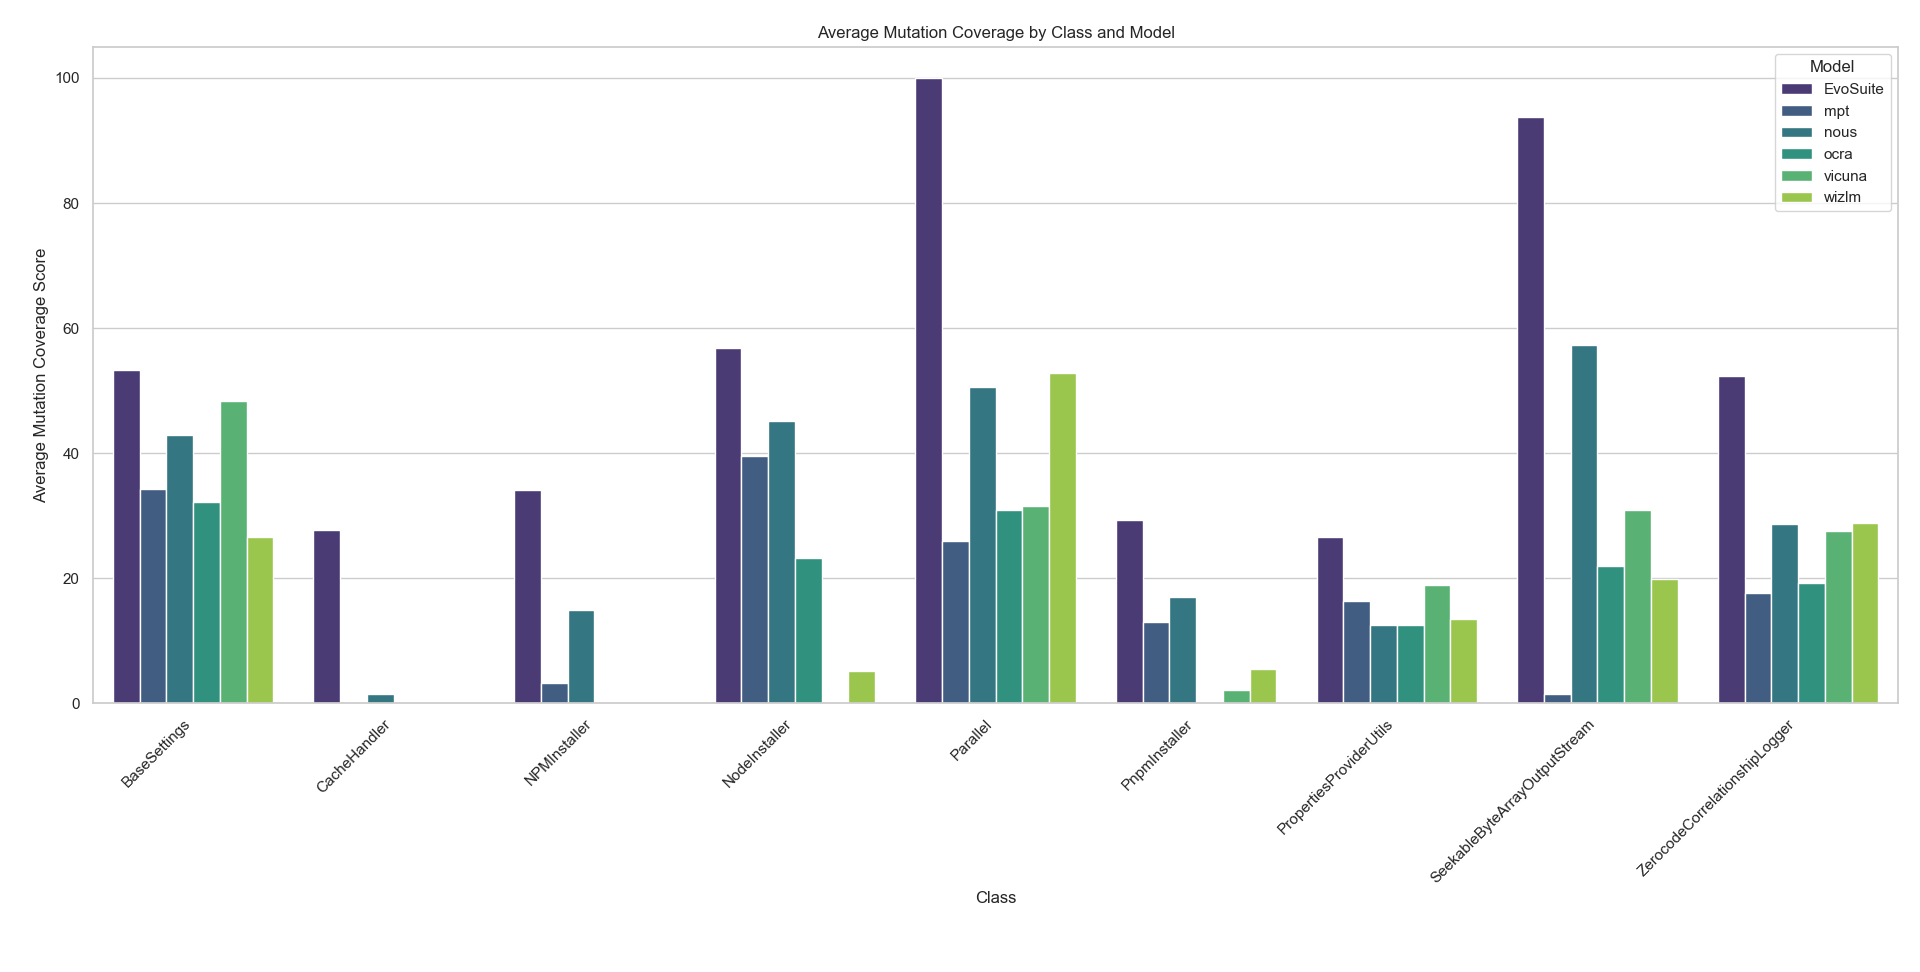
\includegraphics[width=1\textwidth]{images/mutation_coverage_avg.png}
\caption{Average Mutation Coverage by Class and Models}
\label{fig:mutation_coverage}
\end{figure}

\begin{figure}[H]
\centering
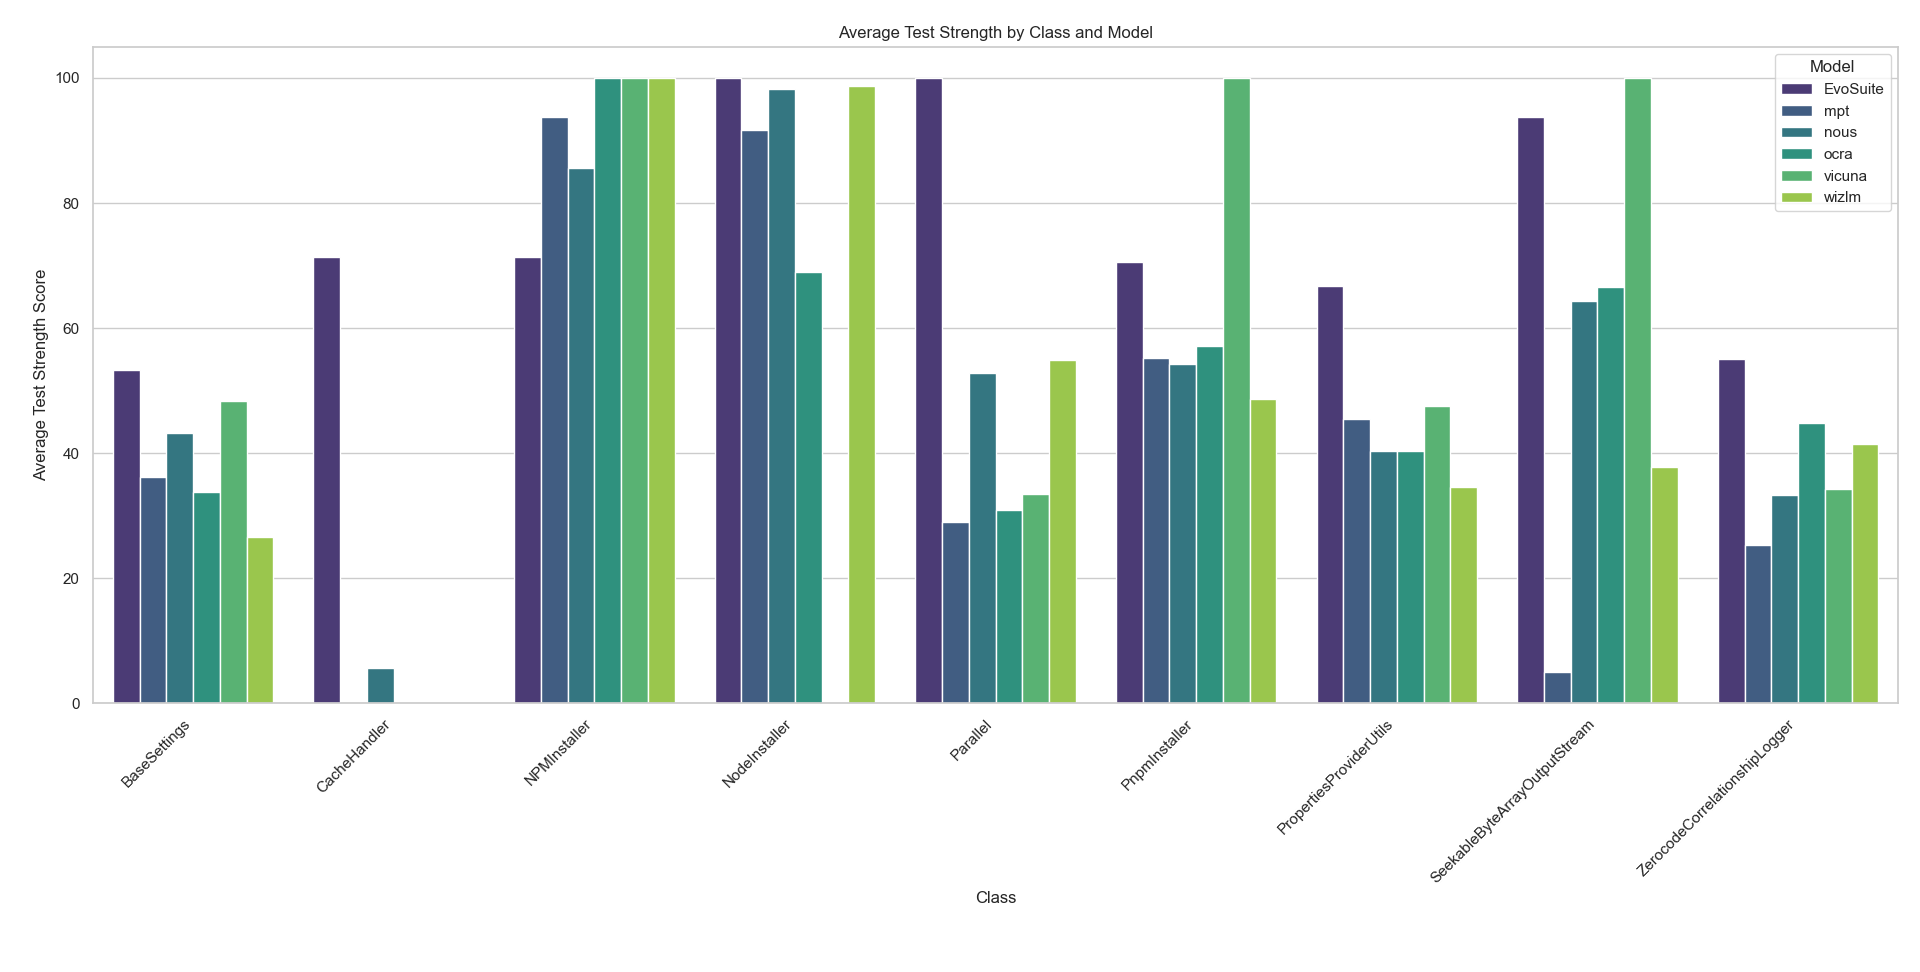
\includegraphics[width=1\textwidth]{images/test_strength_avg.png}
\caption{Average Test Strength by Class and Models}
\label{fig:test_strength}
\end{figure}

\begin{figure}[H]
\centering
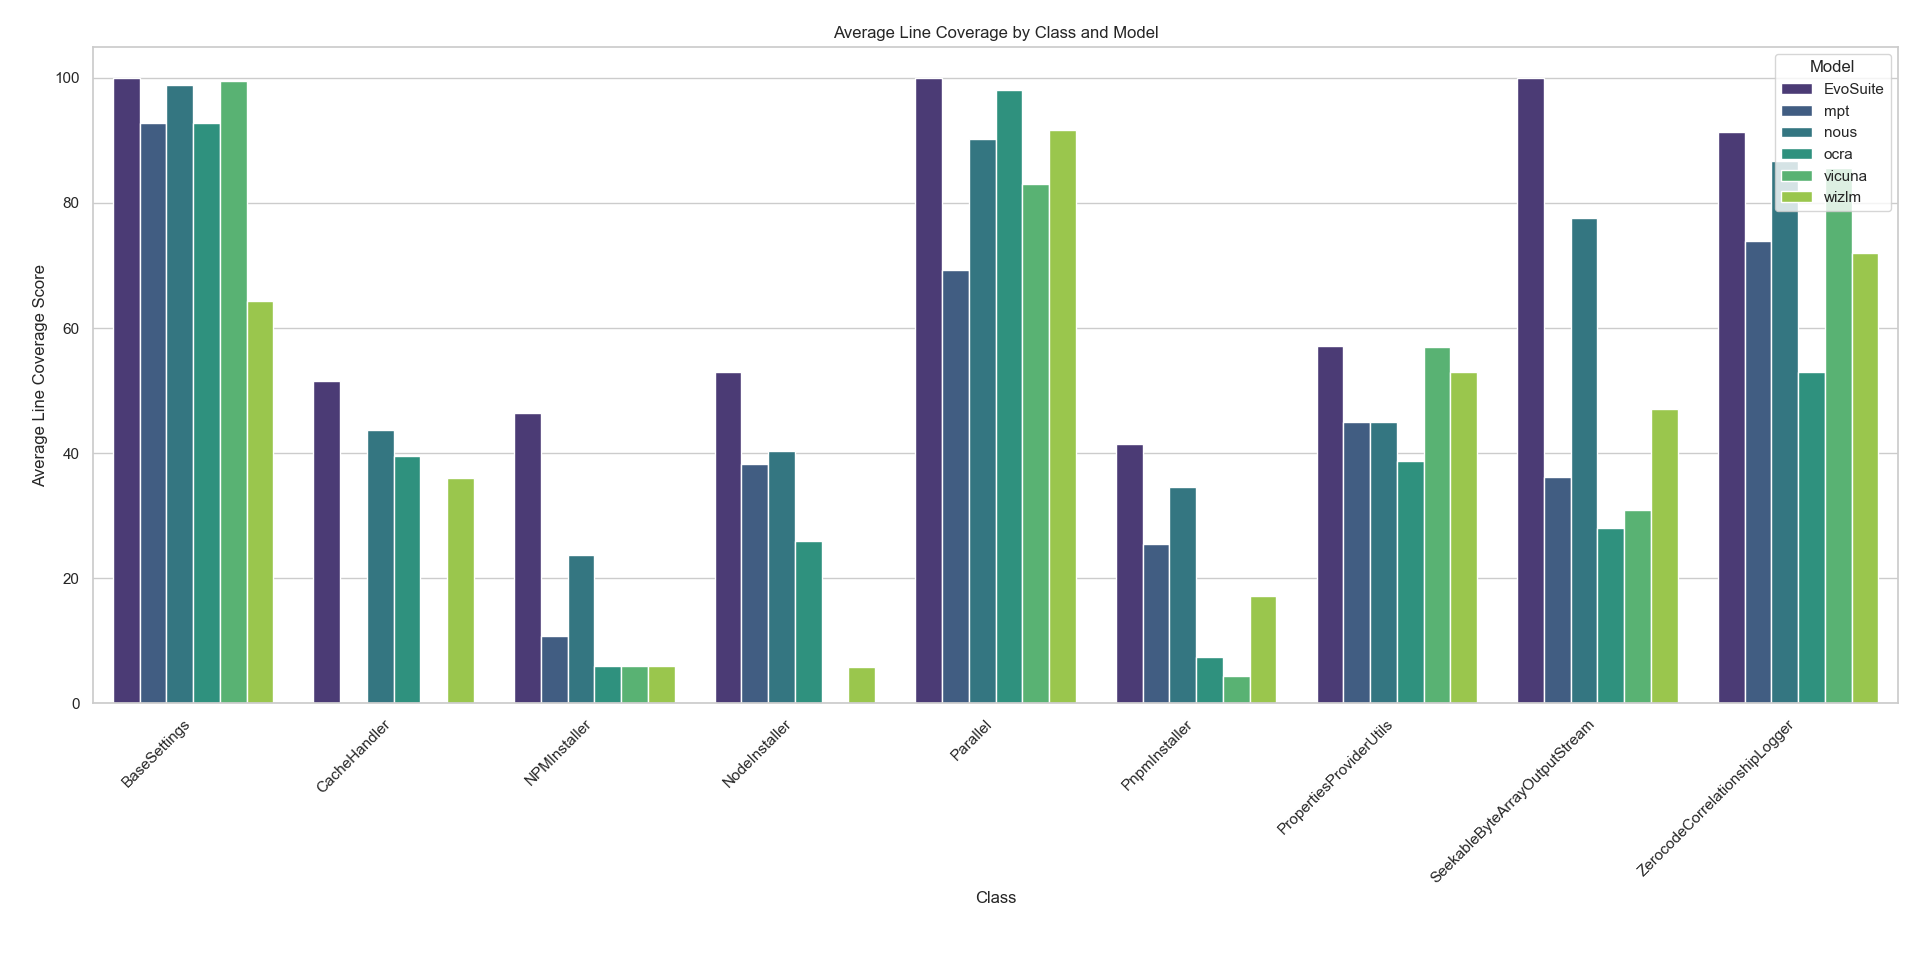
\includegraphics[width=1\textwidth]{images/line_coverage_avg.png}
\caption{Average Line Coverage by Class and Models}
\label{fig:line_coverage}
\end{figure}

\begin{figure}[H]
\centering
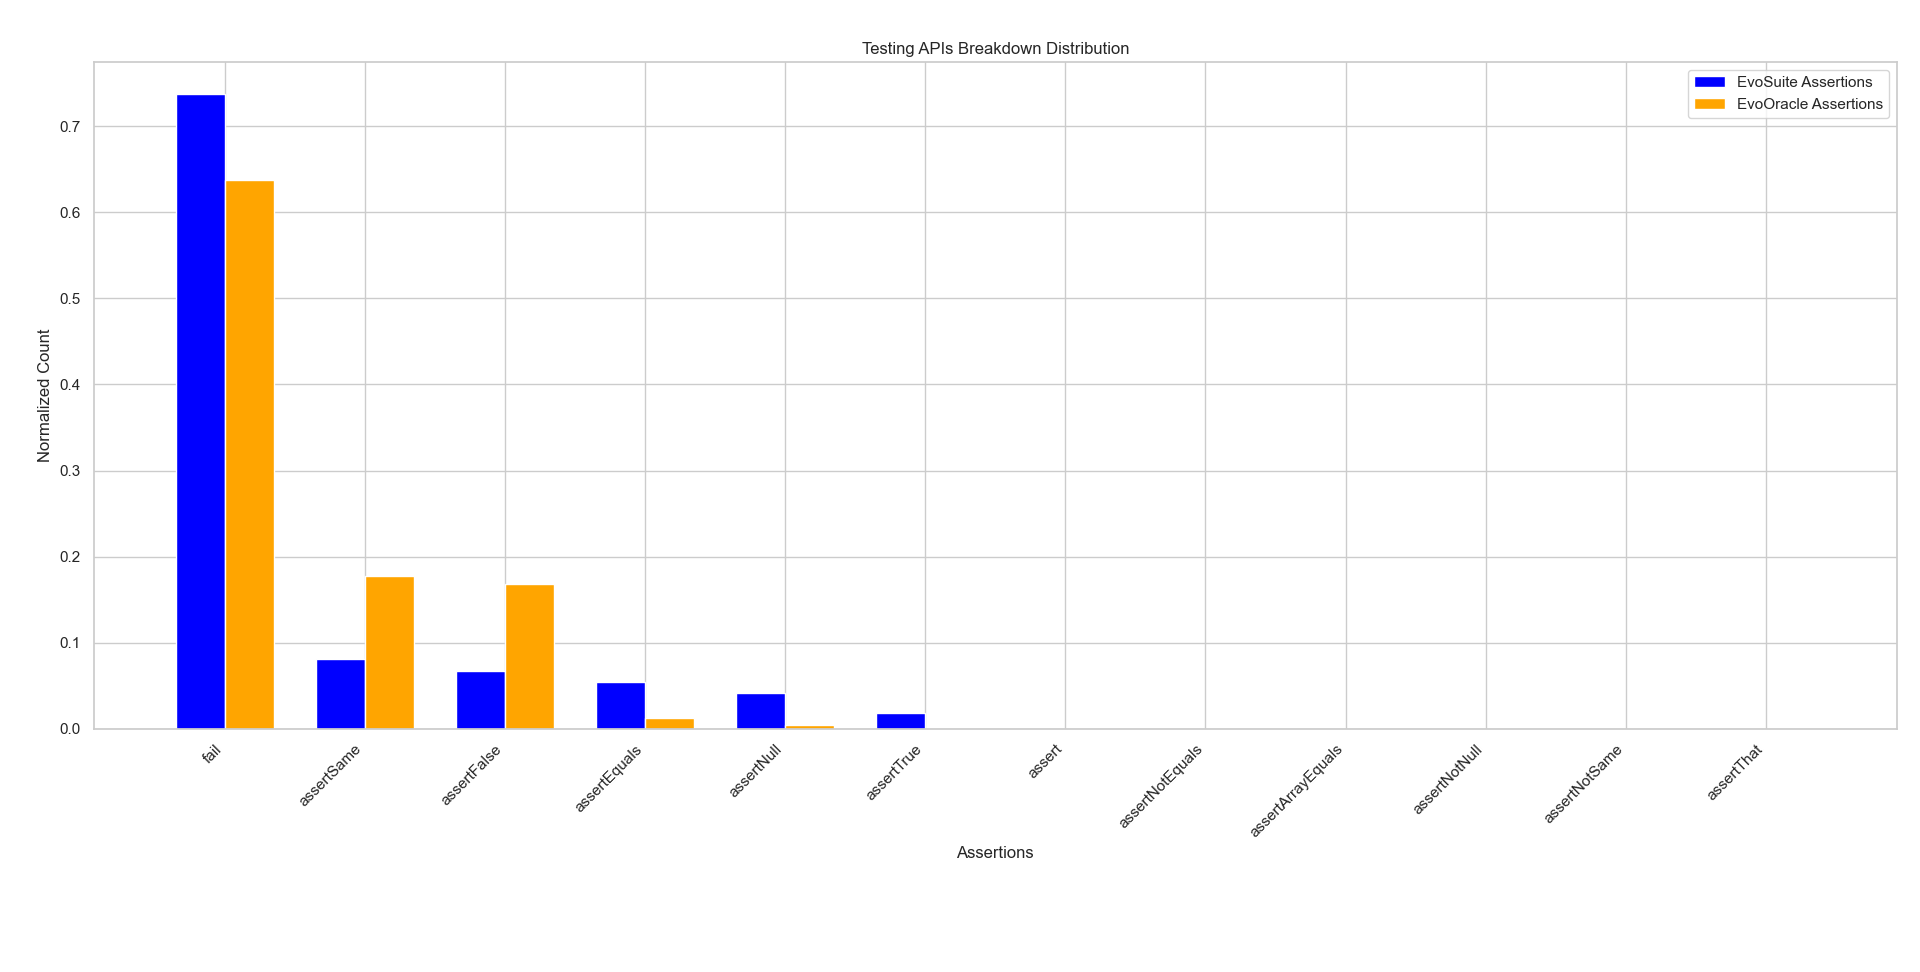
\includegraphics[width=1\textwidth]{images/test_api_distribution.png}
\caption{Testing APIs Breakdown Distribution: EvoSuite vs EvoOracle}
\label{fig:test_api_distribution}
\end{figure}

\begin{figure}[H]
\centering
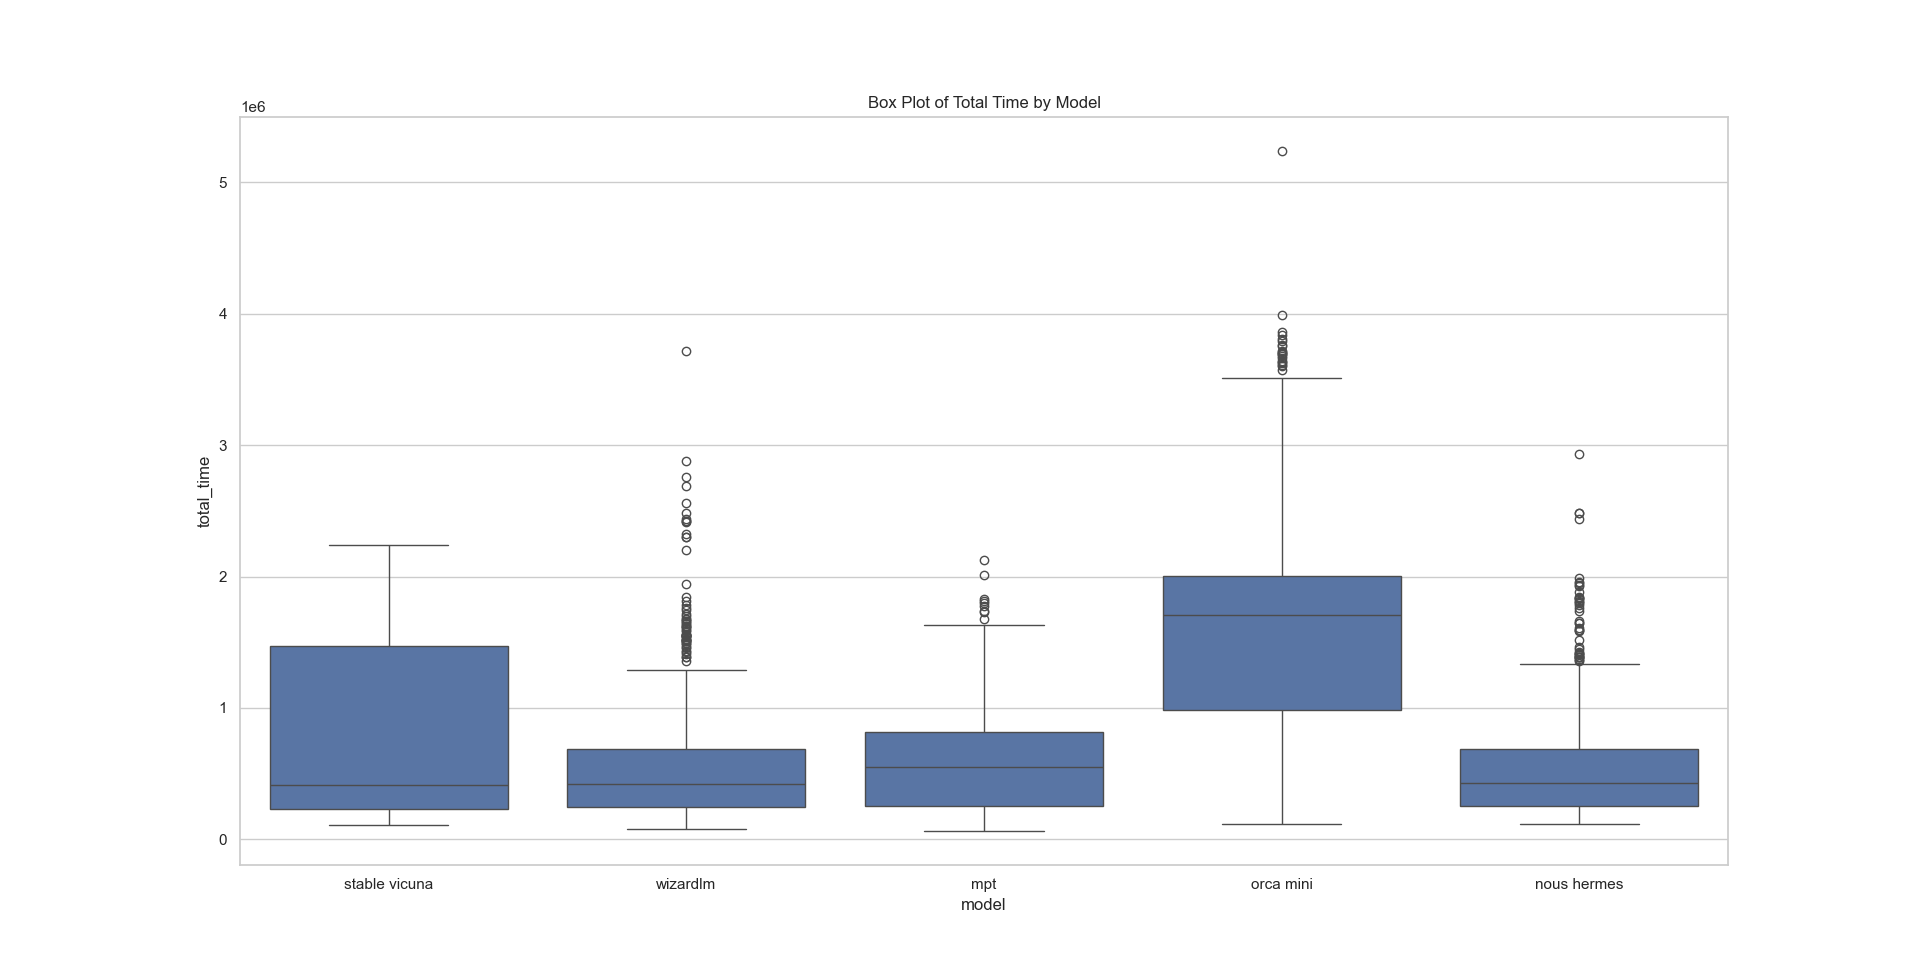
\includegraphics[width=1\textwidth]{images/time_by_model.png}
\caption{Total time taken by Models}
\label{fig:time_models}
\end{figure}

\begin{figure}[H]
\centering
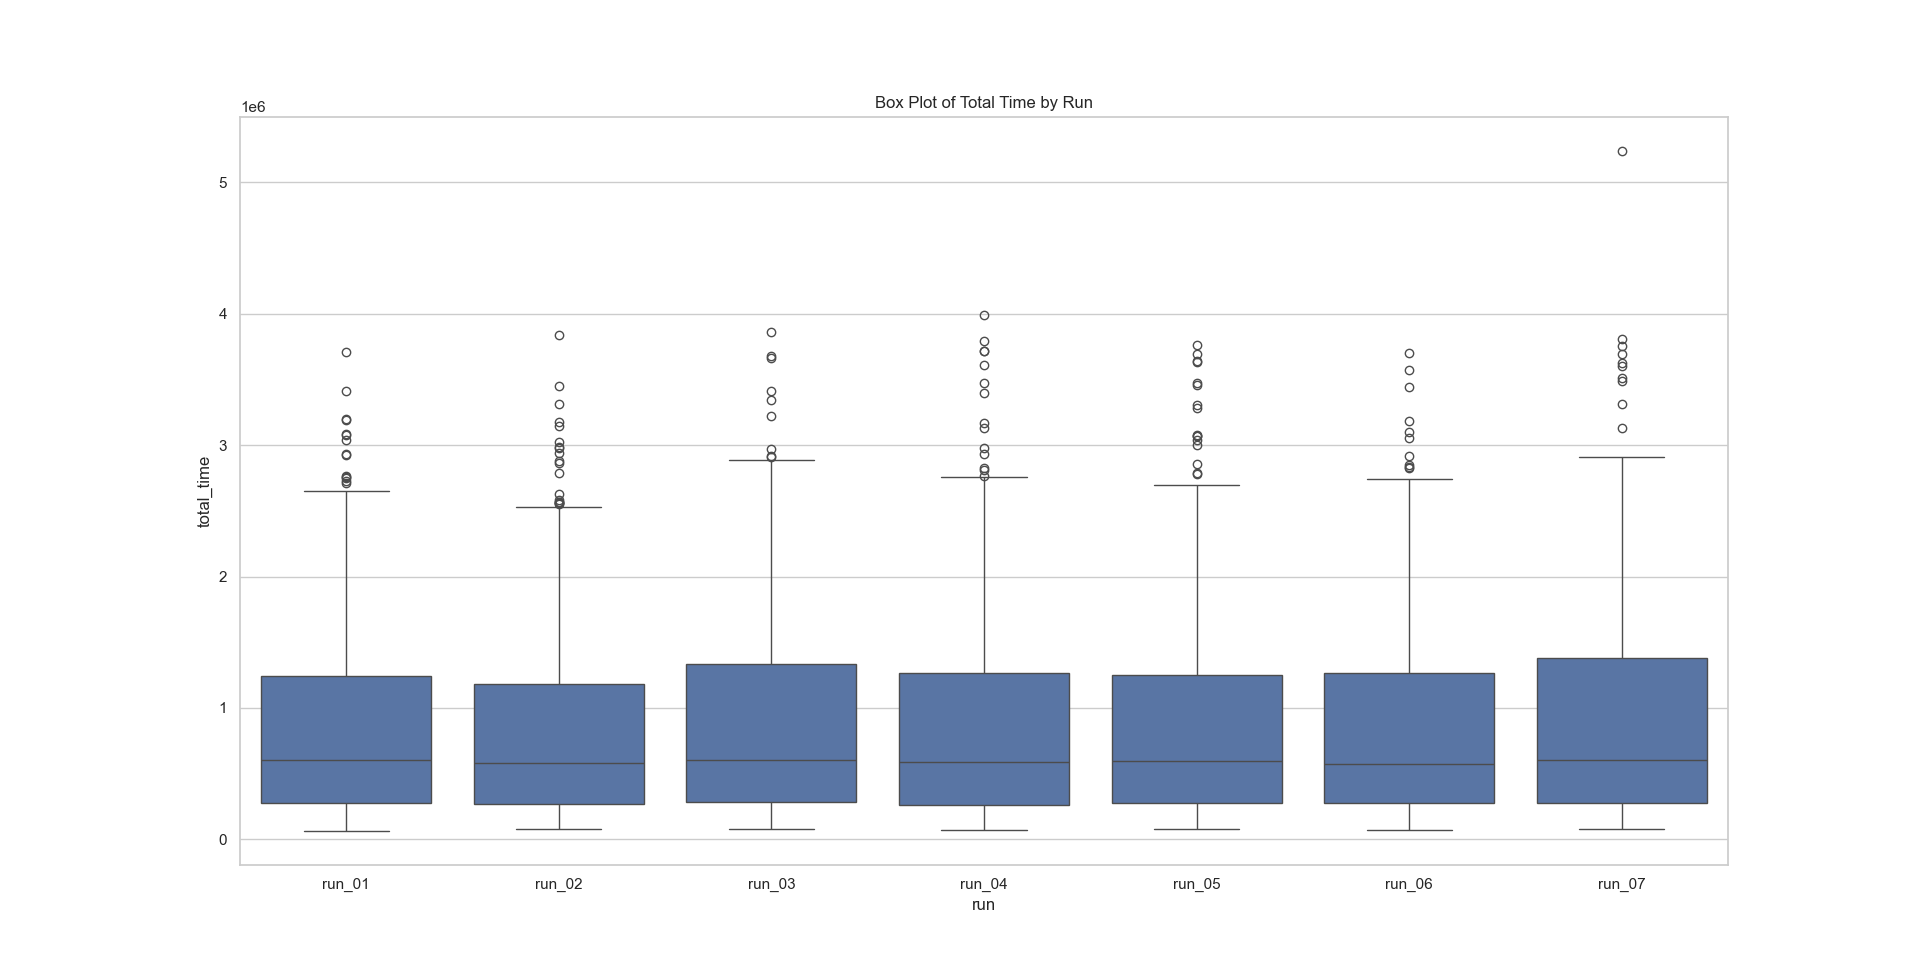
\includegraphics[width=1\textwidth]{images/time_by_runs.png}
\caption{Total time taken by each run}
\label{fig:time_runs}
\end{figure}

\begin{figure}[H]
\centering
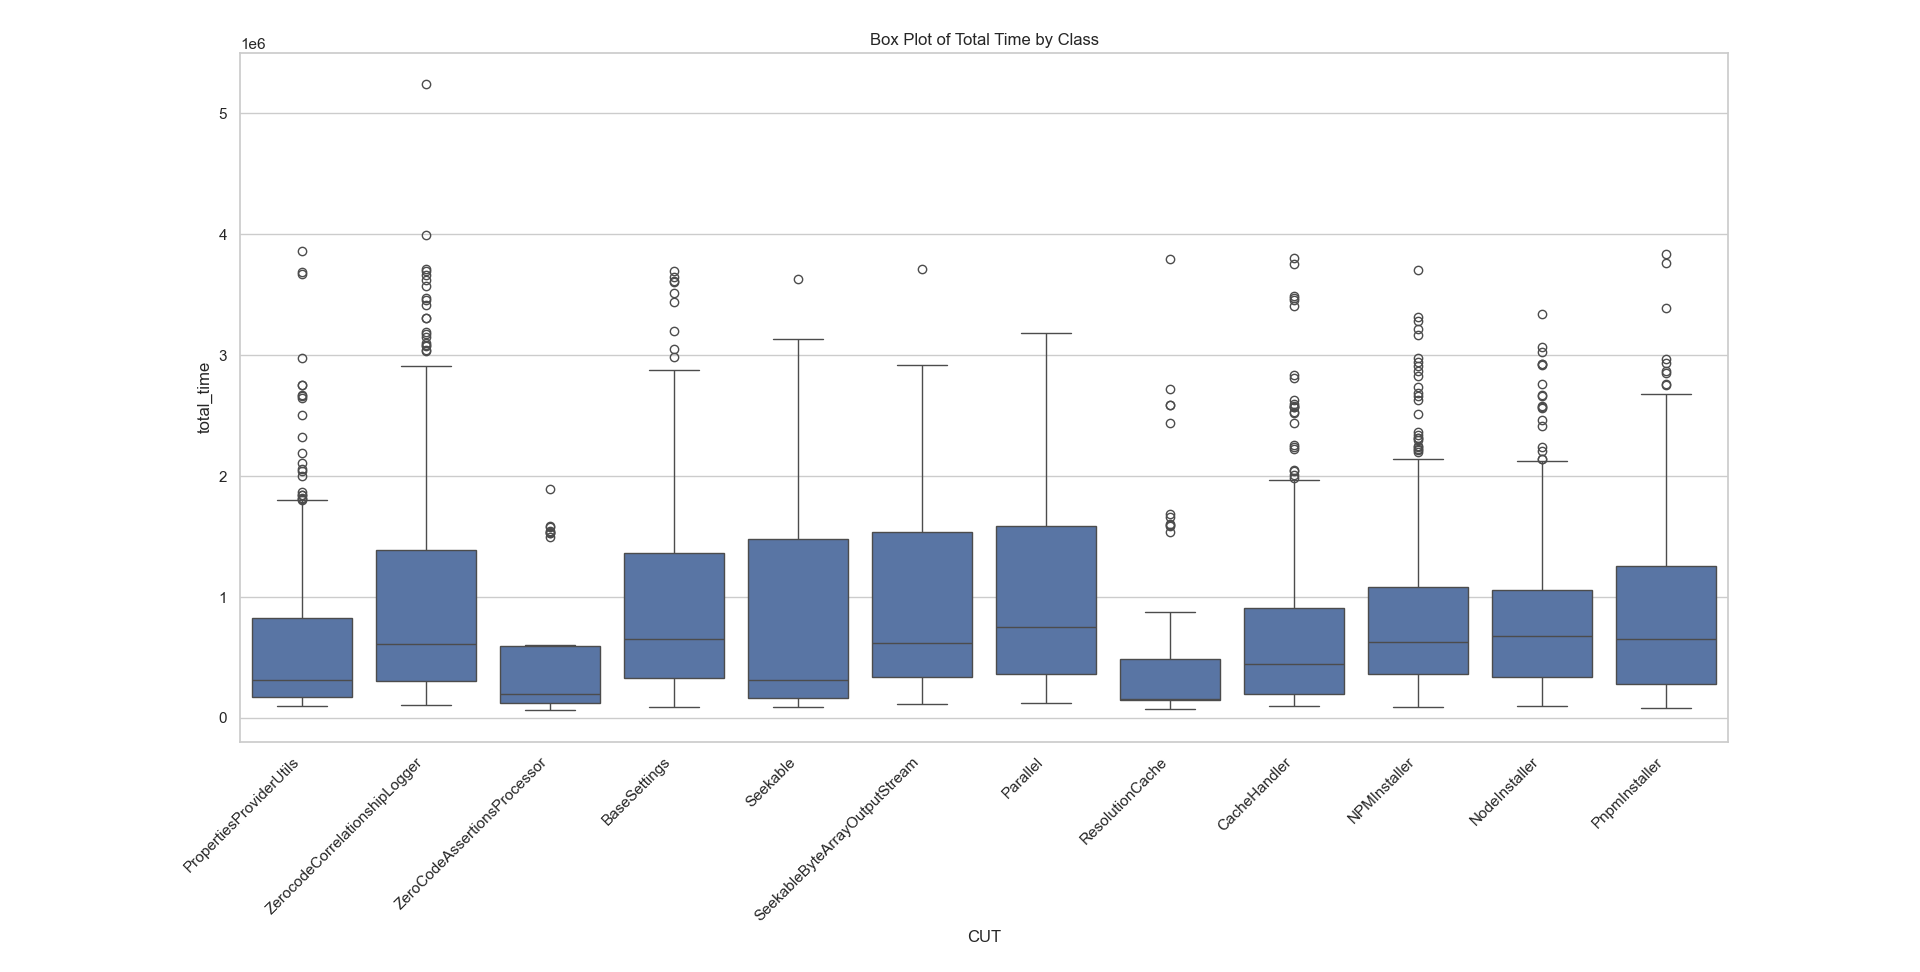
\includegraphics[width=1\textwidth]{images/total_time_by_class.png}
\caption{Total time taken by each class}
\label{fig:time_class}
\end{figure}

\begin{figure}[H]
\centering
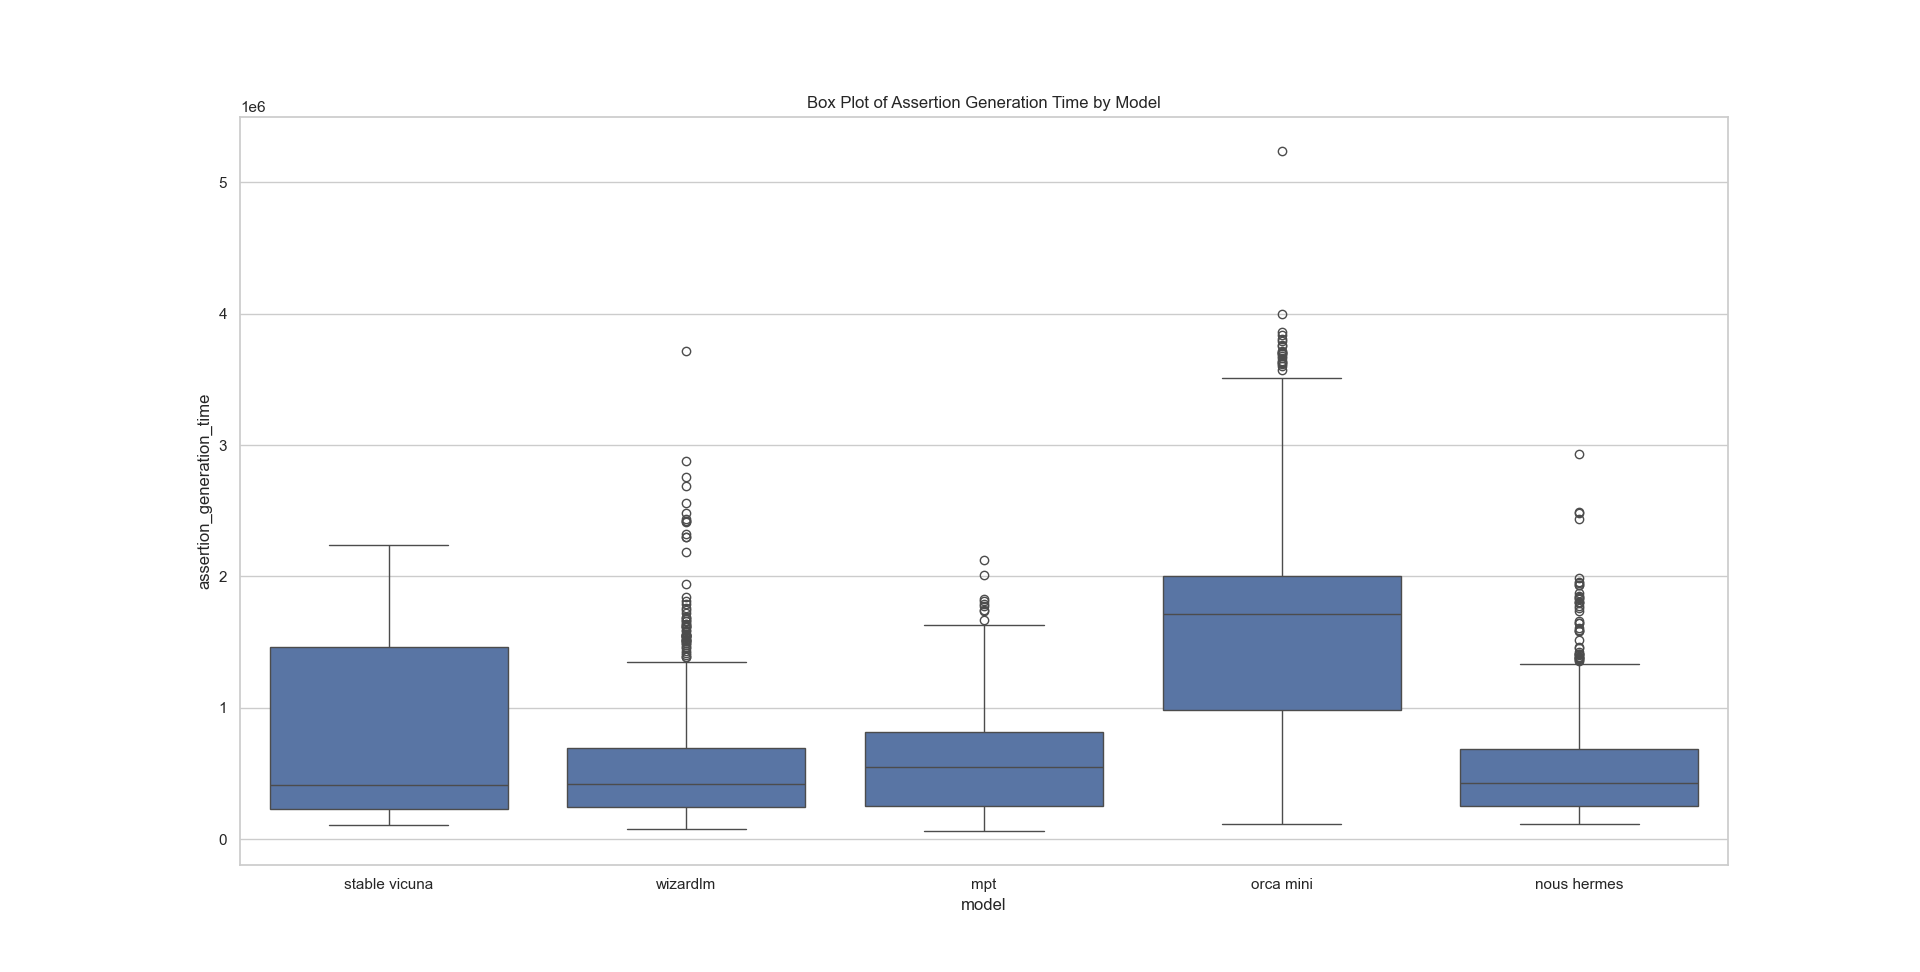
\includegraphics[width=1\textwidth]{images/assertion_time_by_model.png}
\caption{Assertion generation time taken by each model}
\label{fig:assertion_time_models}
\end{figure}

\begin{figure}[H]
\centering
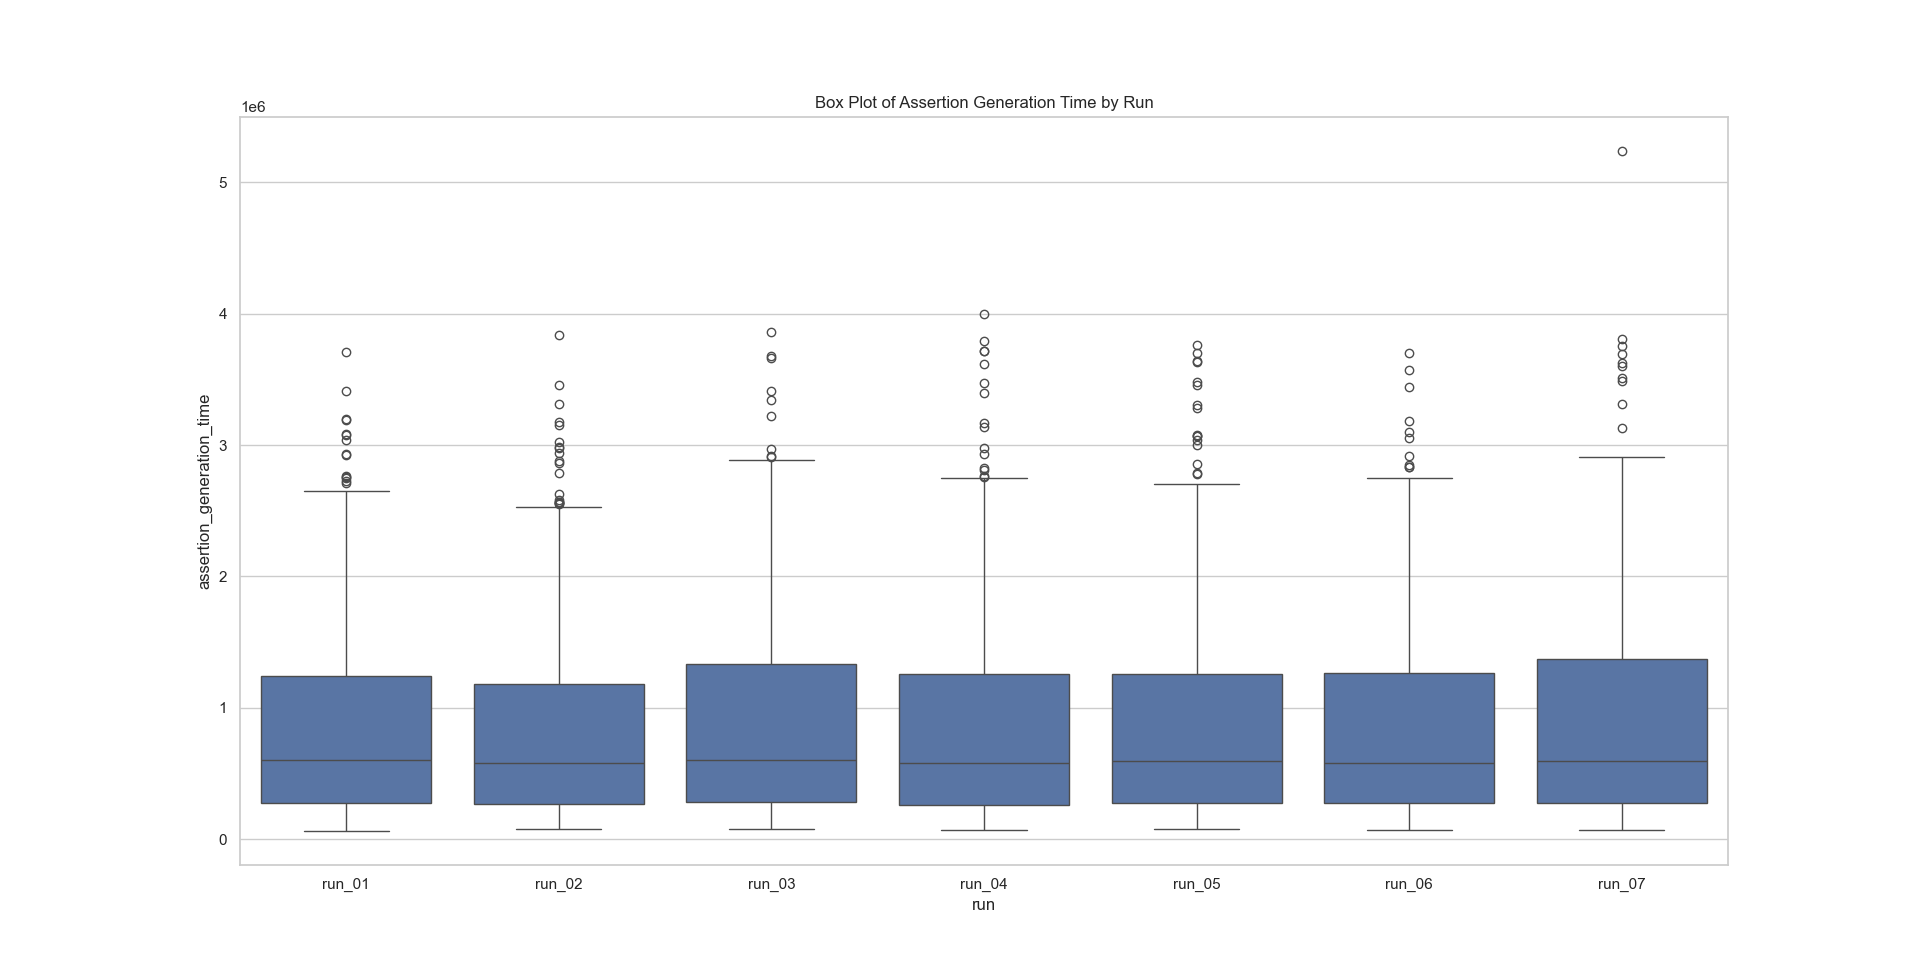
\includegraphics[width=1\textwidth]{images/assertion_time_by_runs.png}
\caption{Assertion generation time taken by each run}
\label{fig:assertion_time_runs}
\end{figure}

\begin{figure}[H]
\centering
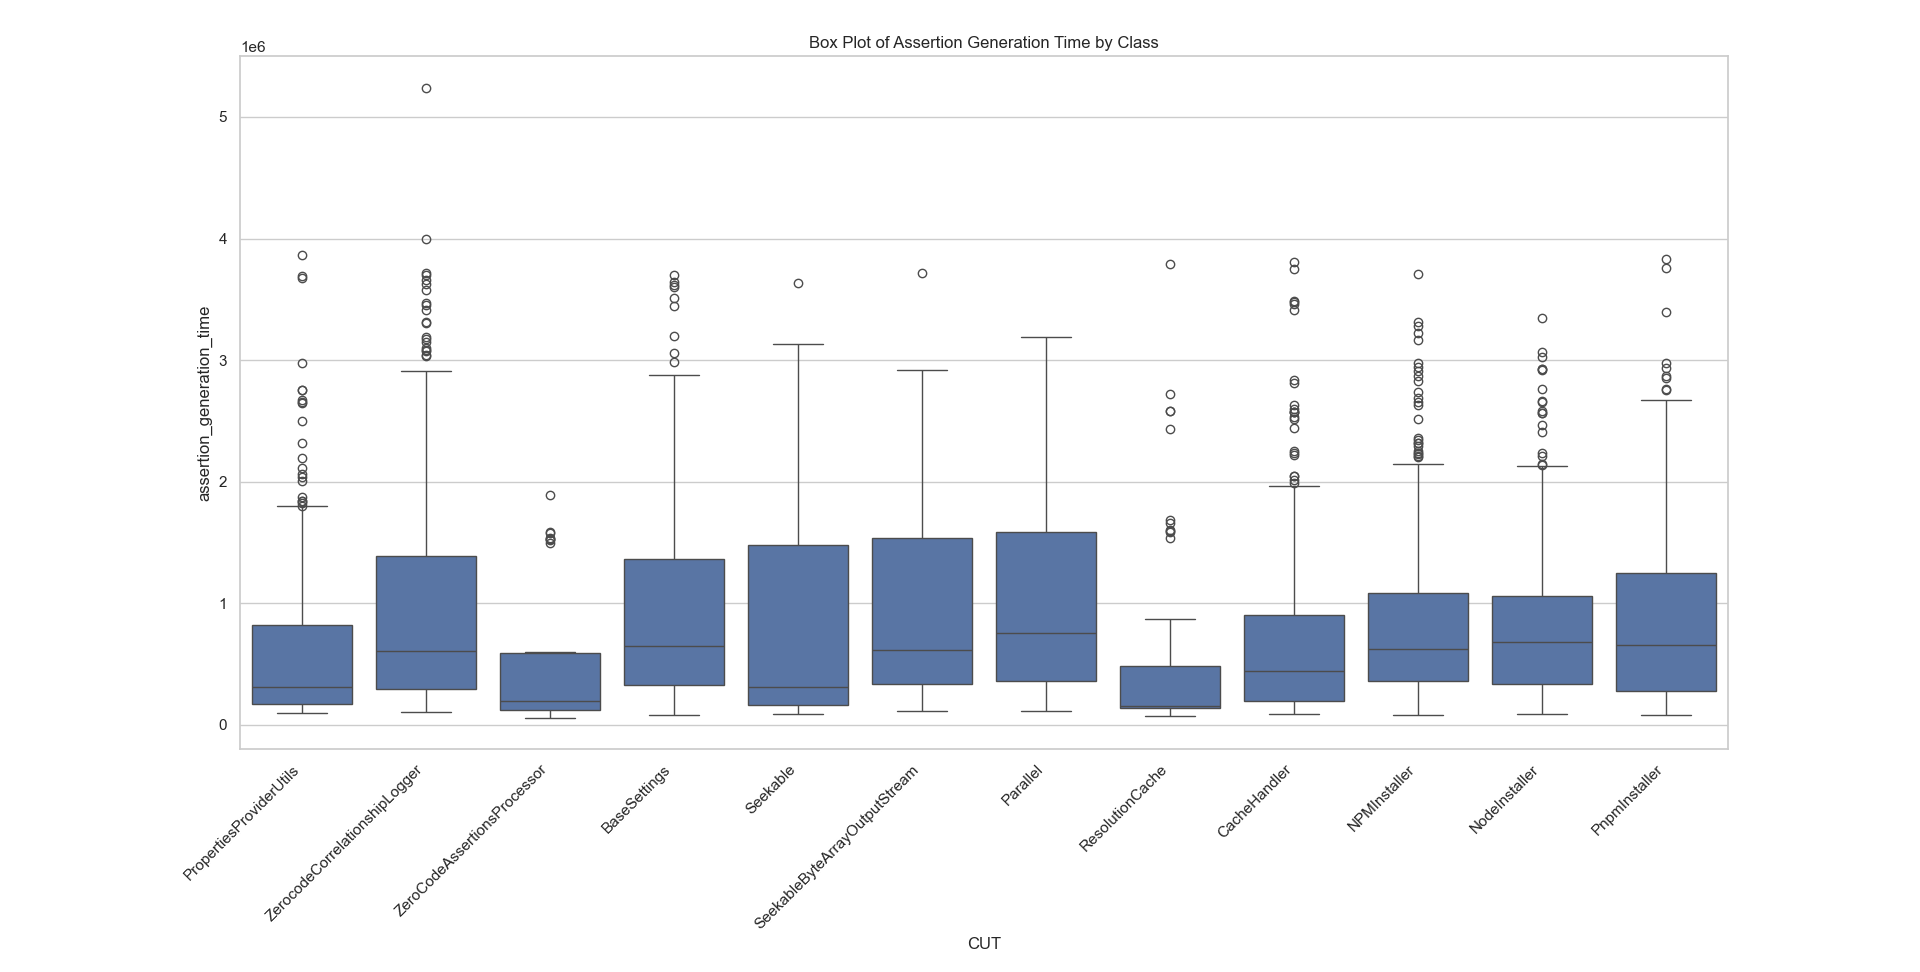
\includegraphics[width=1\textwidth]{images/assertion_time_by_class.png}
\caption{Assertion generation time taken by each class}
\label{fig:assertion_time_class}
\end{figure}

\vspace{0.1 cm}
\subsection{RQ2}
\label{sec:results_rq2}
\vspace{0.1 cm}

In this subsection, an overview of ...

\section{Threats to Validity}
\label{sec:t2v}
\vspace{0.2 cm}

The study acknowledges several potential threats to its validity.

\begin{enumerate}
    \item \textbf{Randomness in LLM Outputs:} One significant threat to the study's validity stems from the inherent randomness associated with Large Language Models (LLMs). The generated outputs are subject to variations based on the model's training conditions and prompt inputs, potentially impacting the reproducibility and consistency of results. In order to minimize the variation, we ran each experiments 7 times and took the median results.

    \item \textbf{Generalizability to Diverse Datasets:} The study recognizes the potential limitation of generalizability to other datasets or programming languages. The findings, rooted in the analysis of Java projects from GitHub, may not extend seamlessly to different programming communities or languages, highlighting a domain-specific consideration.

    \item \textbf{Dataset-Induced Bias:} The dataset itself, composed of Java projects sourced from GitHub, introduces a possible bias reflective of the practices and characteristics specific to the Java programming community on this platform. This inherent bias could influence the study's conclusions and their applicability to broader software development contexts.

    \item \textbf{Concerns of Data Leakage:} In addressing concerns related to data leakage, the study takes precautionary measures by excluding candidate repositories that might appear in the pretraining corpus of the LLMs. This step aims to ensure the integrity of the evaluation process and prevent inadvertent leakage of information.

    \item \textbf{Selection Bias from Compilation and Execution Requirements:} The imposition of specific compilation and execution requirements, such as using Maven as the package manager and ensuring compatibility, introduces a potential source of selection bias. The study acknowledges the impact of these criteria on the composition of the chosen repositories, potentially affecting the representativeness of the dataset.

    \item \textbf{Evaluation Metrics Limitations:} The study recognizes the limitations of the chosen evaluation metrics and criteria. While these metrics provide a quantitative basis for assessment, they may not comprehensively capture the nuanced aspects of LLM-based test oracle generation. This acknowledgment indicates a need for a holistic understanding beyond the quantitative measures employed.
\end{enumerate}

These considerations collectively contribute to the study's robustness and transparency, providing insights into potential factors that may influence the interpretation and application of its findings.

\section{Discussion}
\label{sec:discussion}
\vspace{0.2 cm}

Diving into a comprehensive discussion of our experiments and findings unveils nuanced insights into the intricate landscape of automated testing practices, particularly in the context of leveraging Large Language Models (LLMs) for test oracle generation. The empirical analysis of our approach to generating oracles for unit test cases provides a nuanced understanding of the challenges and potential breakthroughs in this domain. As we navigate the landscape of automated testing, it becomes evident that the multifaceted nature of test cases poses unique challenges that demand innovative solutions.

The comparative analysis between LLM-generated assertions and traditional automated test generation tools, exemplified by EvoSuite, brings to light unexpected and valuable results. The effectiveness and efficiency of LLM-based approaches did not universally outperform traditional methods, marking a noteworthy observation that prompts a deeper exploration into the factors influencing assertion quality and the overall testing workflow.

Surprisingly, LLMs, despite their profound capabilities in understanding natural language, grapple with the complexity of translating this understanding into precise code-related tasks. This observation raises critical questions about the adaptability of LLMs to the diverse nature of test cases, each with its unique intricacies and requirements for meaningful assertions. As developers interact with LLM-generated assertions, a spectrum of sentiments emerges, reflecting the potential and challenges in incorporating advanced language models into the day-to-day software development processes.

Moreover, the results of Research Question 2, indicating an average time of 8.24 minutes for assertion generation for a single test case, shed light on a usability challenge. This prompts considerations about real-world practicality, prompting us to explore alternative approaches, including leveraging APIs like ChatGPT\cite{chatgpt}, Bard\cite{bard}, GooseAI\cite{gooseai}, Cohere\cite{cohere}, Claude\cite{claude}, LLaMA\cite{LLaMA}, PaLM\cite{palm} for faster and potentially more efficient interactions.

It's important to highlight that the models utilized in our experiments are general-purpose Large Language Models\cite{}, not specifically fine-tuned for code generation like Codex\cite{finnie-ansley_robots_2022}. Consequently, precise and thoughtful prompting is crucial when engaging with these models. Since they lack specialized training for code-related tasks, providing clear and context-rich instructions becomes paramount to ensure accurate and relevant responses. This characteristic underscores the need for developers to be mindful of the model's general nature and adapt their prompts accordingly for optimal results in the context of code-related inquiries.
      \newpage
      \afterpage{\null\thispagestyle{empty}\clearpage}

      \chapter{Conclusions}
\label{cha:conclusions}
\vspace{0.4 cm}

The conclusion goes here...

The thesis addressed the following research questions:
\begin{enumerate}
  \item RQ1?
  \item RQ2?
\end{enumerate}
By addressing these research questions, this thesis advances knowledge in ...

The main results of the thesis can be summarized as follows:
\begin{itemize}
  \item Result 1
  \item Result 2
\end{itemize}

... proposed in Chapter~\ref{cha:introduction}. This solution would allow ...
      \newpage
      % \afterpage{\null\thispagestyle{empty}\clearpage}

    \endgroup

    % bibliography - bibtex format
    %
    % add chapter to index
    %\addcontentsline{toc}{chapter}{Bibliography}
    % alphabetical order of authors
    %\bibliographystyle{plain}
    %\bibliography{bibliography}
    \printbibliography[heading=bibintoc, title={Bibliography}]

%%%%%%%%%%%%%%%%%%%%%%%%%%%%%%%%%%%%%%%%%%%%%%%%%%%%%%%%%%%%%%%%%%%%%%%%%%
%%%%%%%%%%%%%%%%%%%%%%%%%%%%%%%%%%%%%%%%%%%%%%%%%%%%%%%%%%%%%%%%%%%%%%%%%%
%% Nota
%%%%%%%%%%%%%%%%%%%%%%%%%%%%%%%%%%%%%%%%%%%%%%%%%%%%%%%%%%%%%%%%%%%%%%%%%%
%% In the bibliography, all the sources consulted for the dissertation 
%% have to be cited and listed in alphabetical order by the 
%% first author's surname.
%%
%% According to the source material, the quotation has to be as follows:
%%
%% BOOKS
%% Surname and initial/s of the name/s of the author/s, date of edition,
%% publishing house and (if applicable) number of edition.
%% 
%% JOURNAL ARTICLES 
%% Surname and initial/s of the first name/s of the author/s,
%% title of the article, name of the journal, volume number, issue number
%% and page numbers.
%% 
%% CONFERENCE PAPERS
%% Surname and initial/s of the name/s of the author/s,
%% year of the conference, title of the article, name of the conference,
%% place of the conference, conference dates, page numbers.
%% 
%% CITING WEB RESOURCES
%% The consulted webpages have to be listed in alphabetical order. 
%% It is necessary to:
%%   - Copy the specific URL (the web address) of the consulted webpage
%%   - If available, indicate the surname and first name of the author/s,
%%     the title and subtitle of the text
%%   - If available, indicate the last date you retrieved the webpage
%%     (day/month/year).   
%%%%%%%%%%%%%%%%%%%%%%%%%%%%%%%%%%%%%%%%%%%%%%%%%%%%%%%%%%%%%%%%%%%%%%%%%%
%%%%%%%%%%%%%%%%%%%%%%%%%%%%%%%%%%%%%%%%%%%%%%%%%%%%%%%%%%%%%%%%%%%%%%%%%%
    

    %\titleformat{\chapter}
    %    {\normalfont\Huge\bfseries}{Appendix \thechapter}{1em}{}
    % Appendix / attachment section - optional
    %\appendix
    %\chapter{Title of the first attachment}
\label{cha:attach1}
\vspace{0.4 cm}

The first attachment


\section{Title1}
\label{cha:title1}
\vspace{0.2 cm}

The title of the first attachment


\vspace{0.1 cm}
\subsection{Subtitle}
\label{cha:subtitle1}
\vspace{0.1 cm}

The subtitle of the first attachment


\chapter{Title of the second attachment}
\label{cha:attach2}
\vspace{0.4 cm}

The second attachment


\section{Title2}
\label{cha:title2}
\vspace{0.2 cm}

The title of the second attachment


\vspace{0.1 cm}
\subsection{Subtitle2}
\label{cha:subtitle2}
\vspace{0.1 cm}

The subtitle of the second attachment


\end{document}
